% !TeX root = ../main.tex

\chapter{制造,组装与测试}
\label{cha:chapter03}
\section{制造与组装}
图\ref{fig:CAD}和图\ref{fig:carbon_fiber}为第一版设计的机身碳纤维板设计图和实物。这里遇到了一些小问题,设计时未完全考虑到加工情况,由于开槽是用刀具铣,因此方形的槽无法加工,角一定是半径等于刀具的圆角。这个问题在第三版设计的时候体现得比较明显,不得不对零件进行了手工处理才能正常组装。
\begin{figure}[H]
  \centering%
  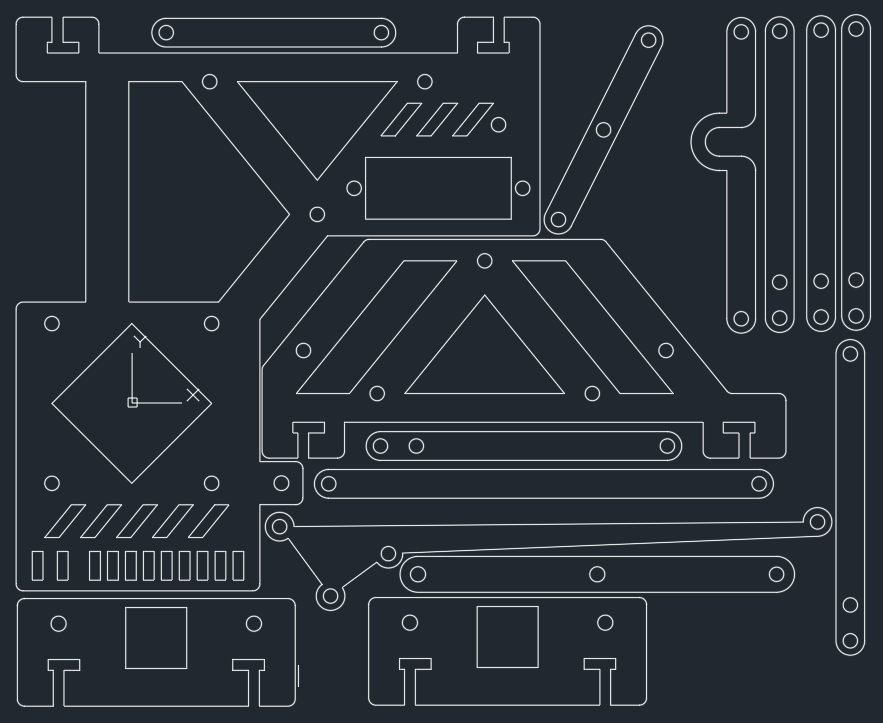
\includegraphics[height=6cm]{CAD.png}
  \caption{CAD设计图(第一版)}
  \label{fig:CAD}
\end{figure}
\begin{figure}[H]
  \centering%
  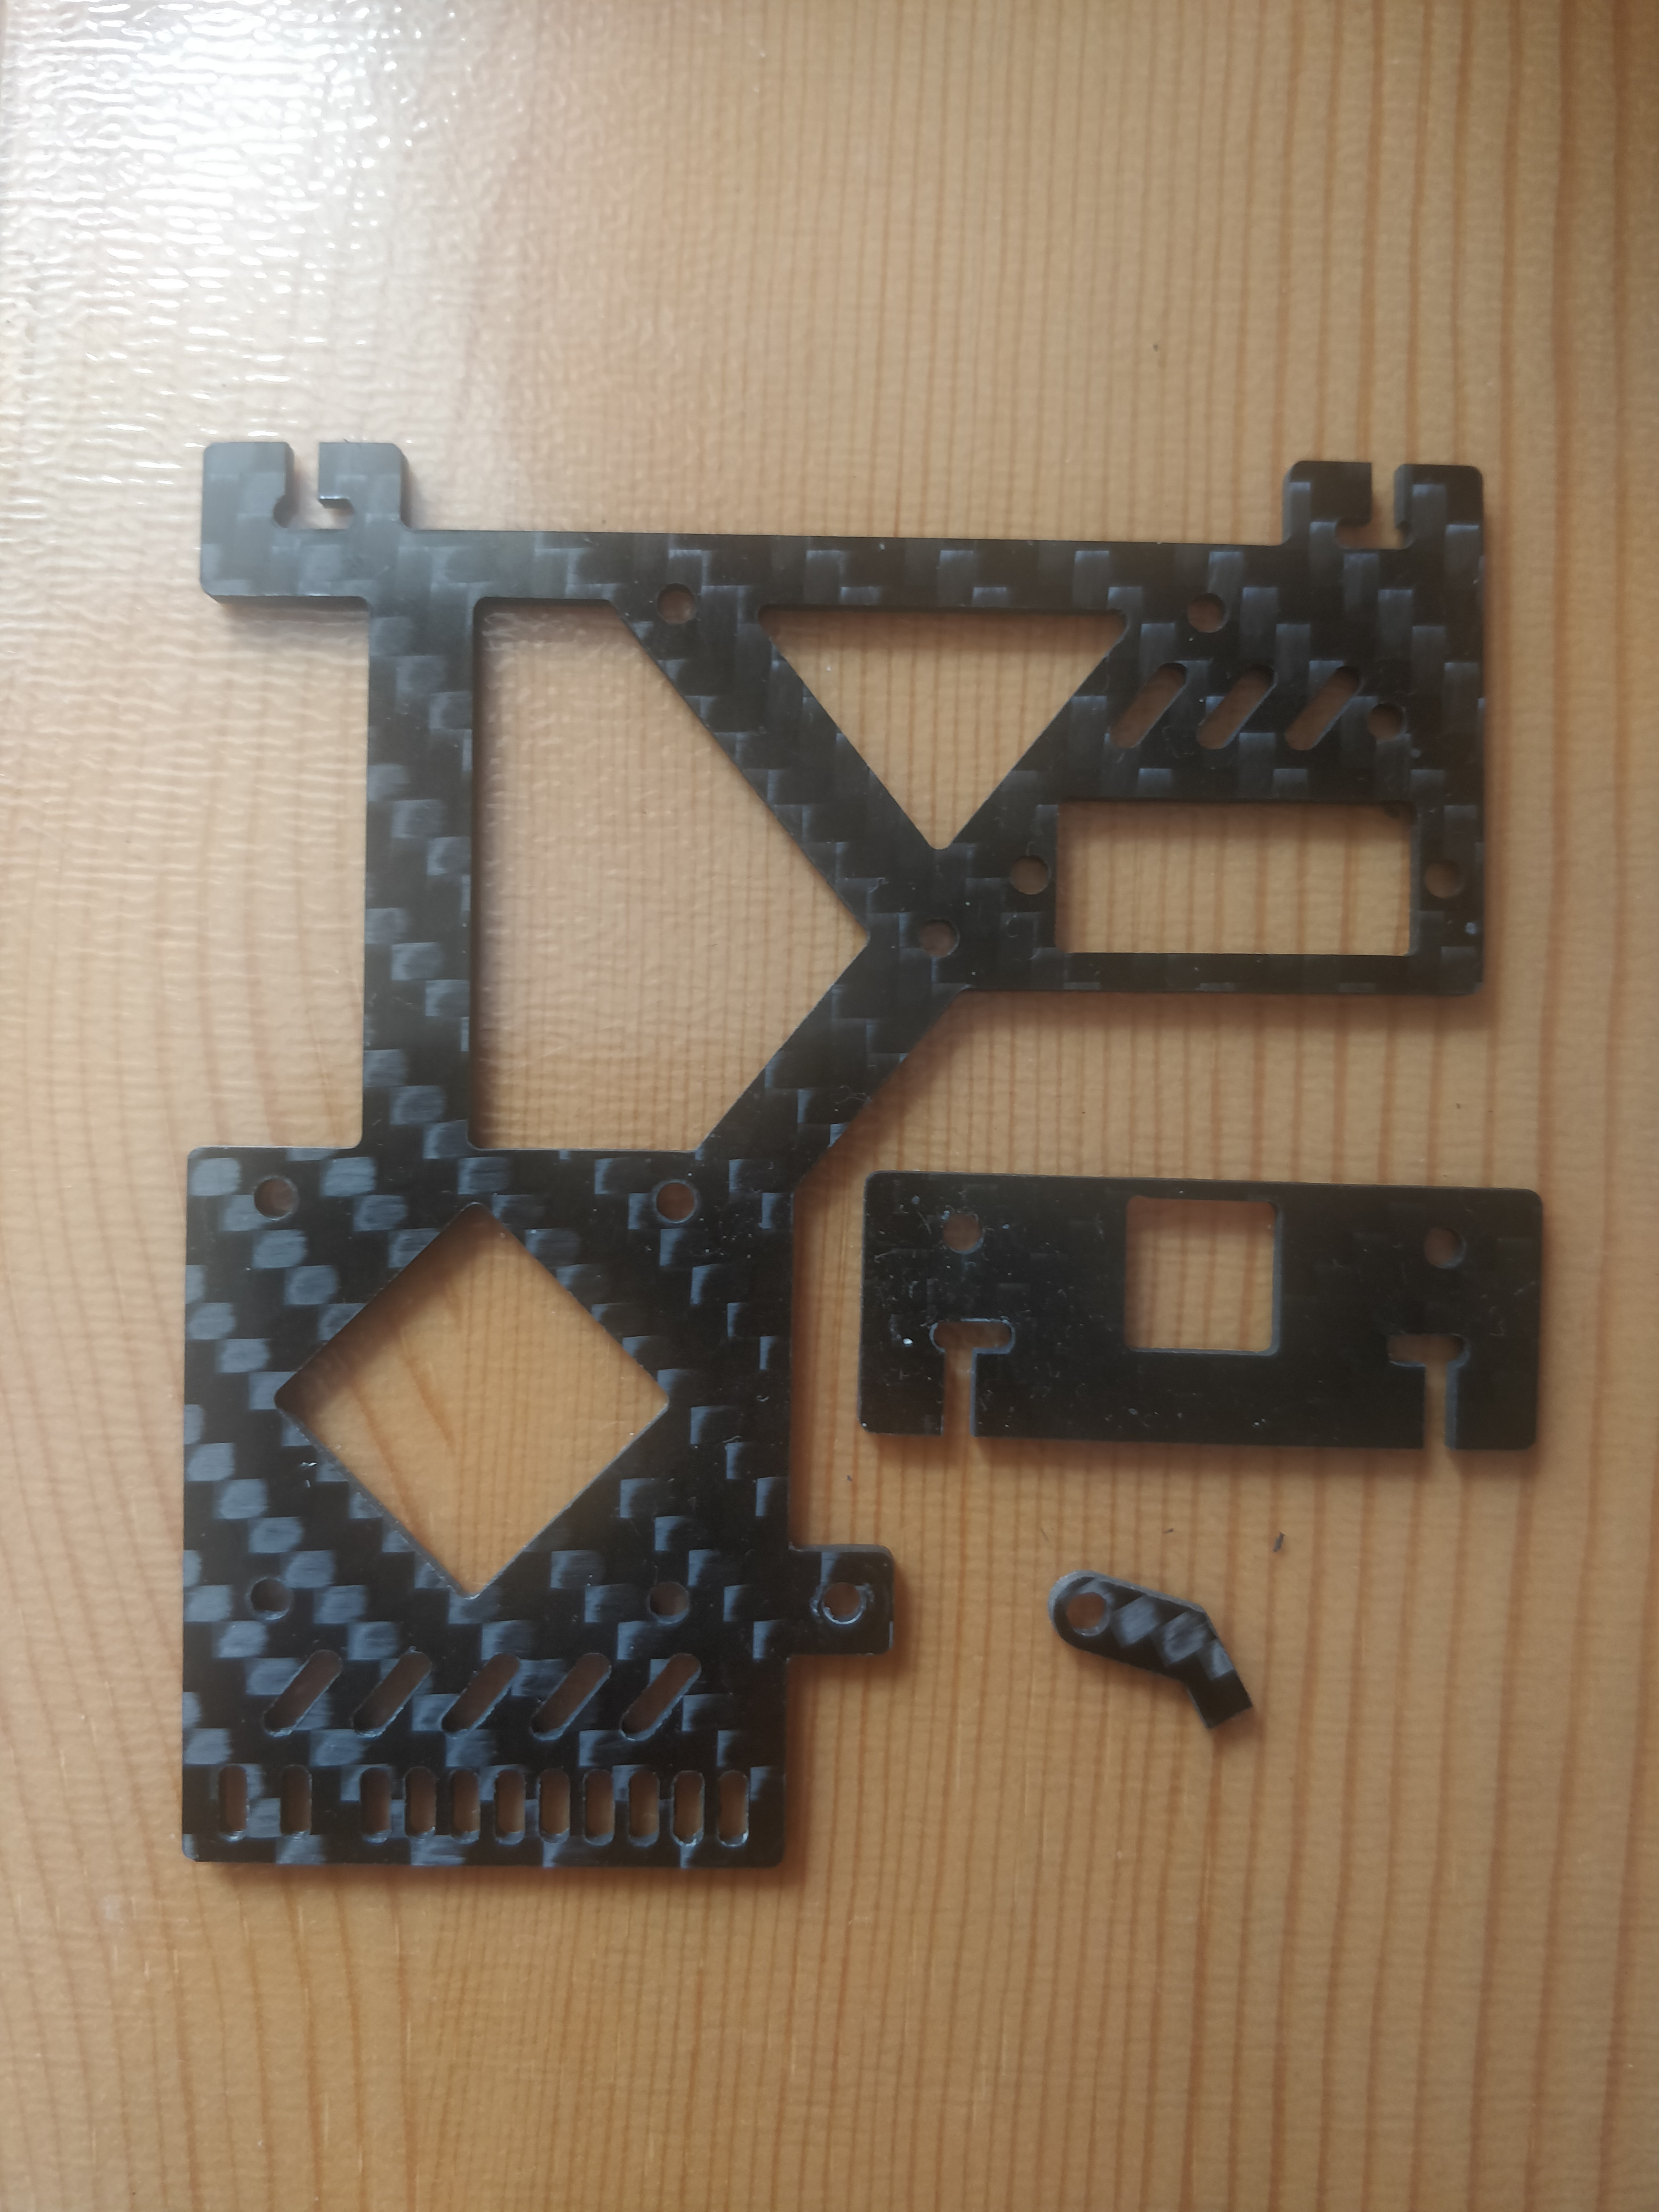
\includegraphics[height=7cm]{carbon_fiber.jpeg}
  \caption{碳纤维切割实物(部分)}
  \label{fig:carbon_fiber}
\end{figure}
机翼接头使用了3D打印ABS材质。这部分也打印了两次,第一次由于不了解选择的商家的3D打印材料的膨胀系数,打印出来的孔都小于要求,商家免费给打印了第二版。虽然第二版有一个零件的孔位依然是错的,以及这次的T型接头断掉了,但自己修修补补勉强都能用(怀疑商家是手动扩的孔)。但最大的问题出在T型接头,3D打印的材料与碳纤维杆之间的摩擦力在舵机拉动时无法忽略,换成铜轴承和滚珠直线轴承也无法解决。因此最终选择增加一个自由度,虽然活动范围有所减小,但满足要求。
\begin{figure}[H]
  \centering%
  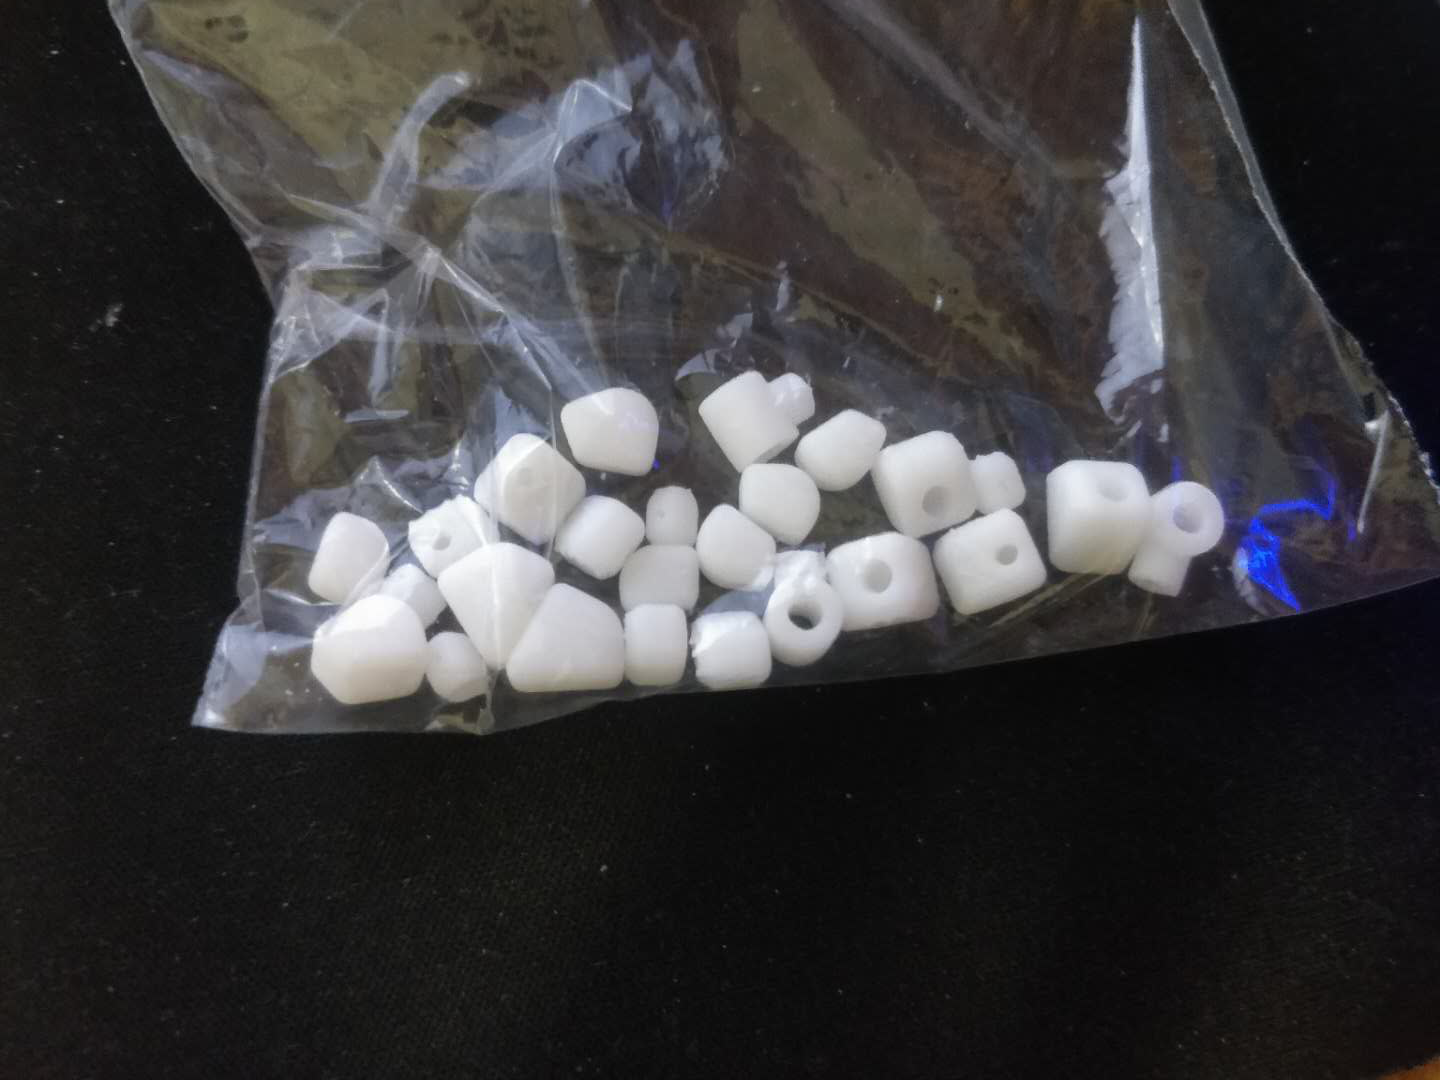
\includegraphics[height=5cm]{3Dprint.png}
  \caption{3D打印零件}
  \label{fig:3Dprint}
\end{figure}
\begin{figure}[H]
  \centering%
  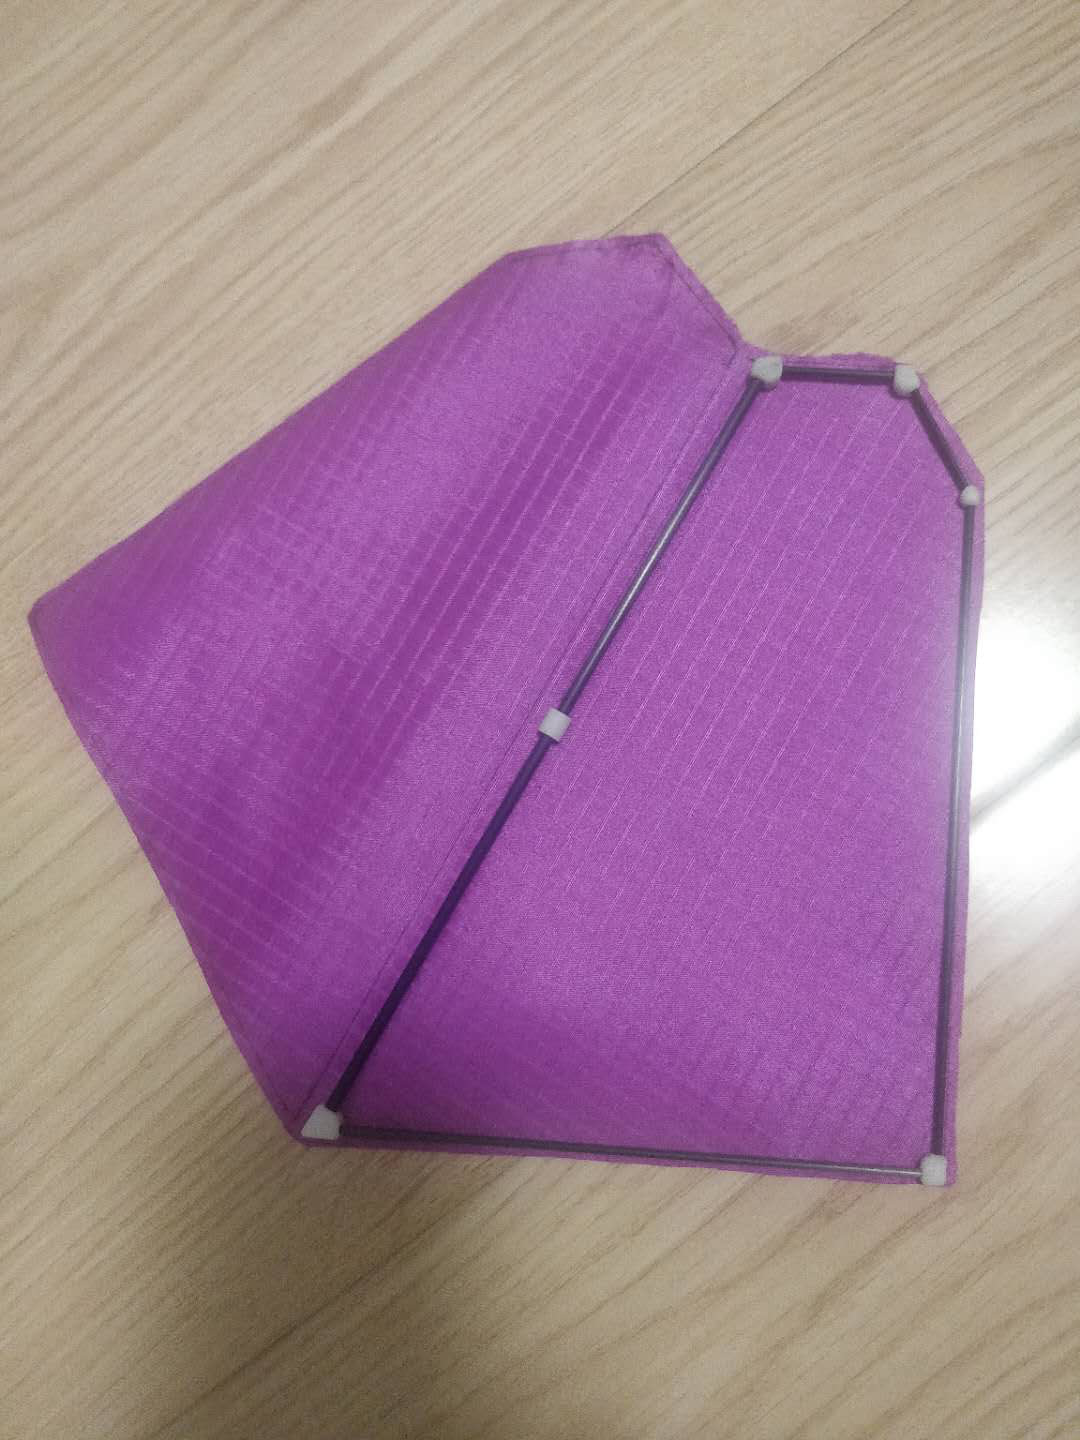
\includegraphics[height=7cm]{wing_assembled.png}
  \caption{机翼组装}
  \label{fig:wing_assembled}
\end{figure}
腿的部分最大的问题来自于元件之间连接的间隙与晃动。设计时各部分是平面设计,连接轴使用了直径2mm的碳纤维杆和金属杆,杆与板的固定使用了卡簧。而实际发现,卡簧径向的摩擦力不够可靠,而且一些关节的晃动会被机构放大,几次运动之后晃动就大到无法接受。因此使用AB胶对关节进行了加固,如图\ref{fig:leg_assembled}所示。但一段时间过后依然会松动,想彻底解决晃动问题需要改变设计(如使用金属材料等)。
\begin{figure}[H]
  \centering%
  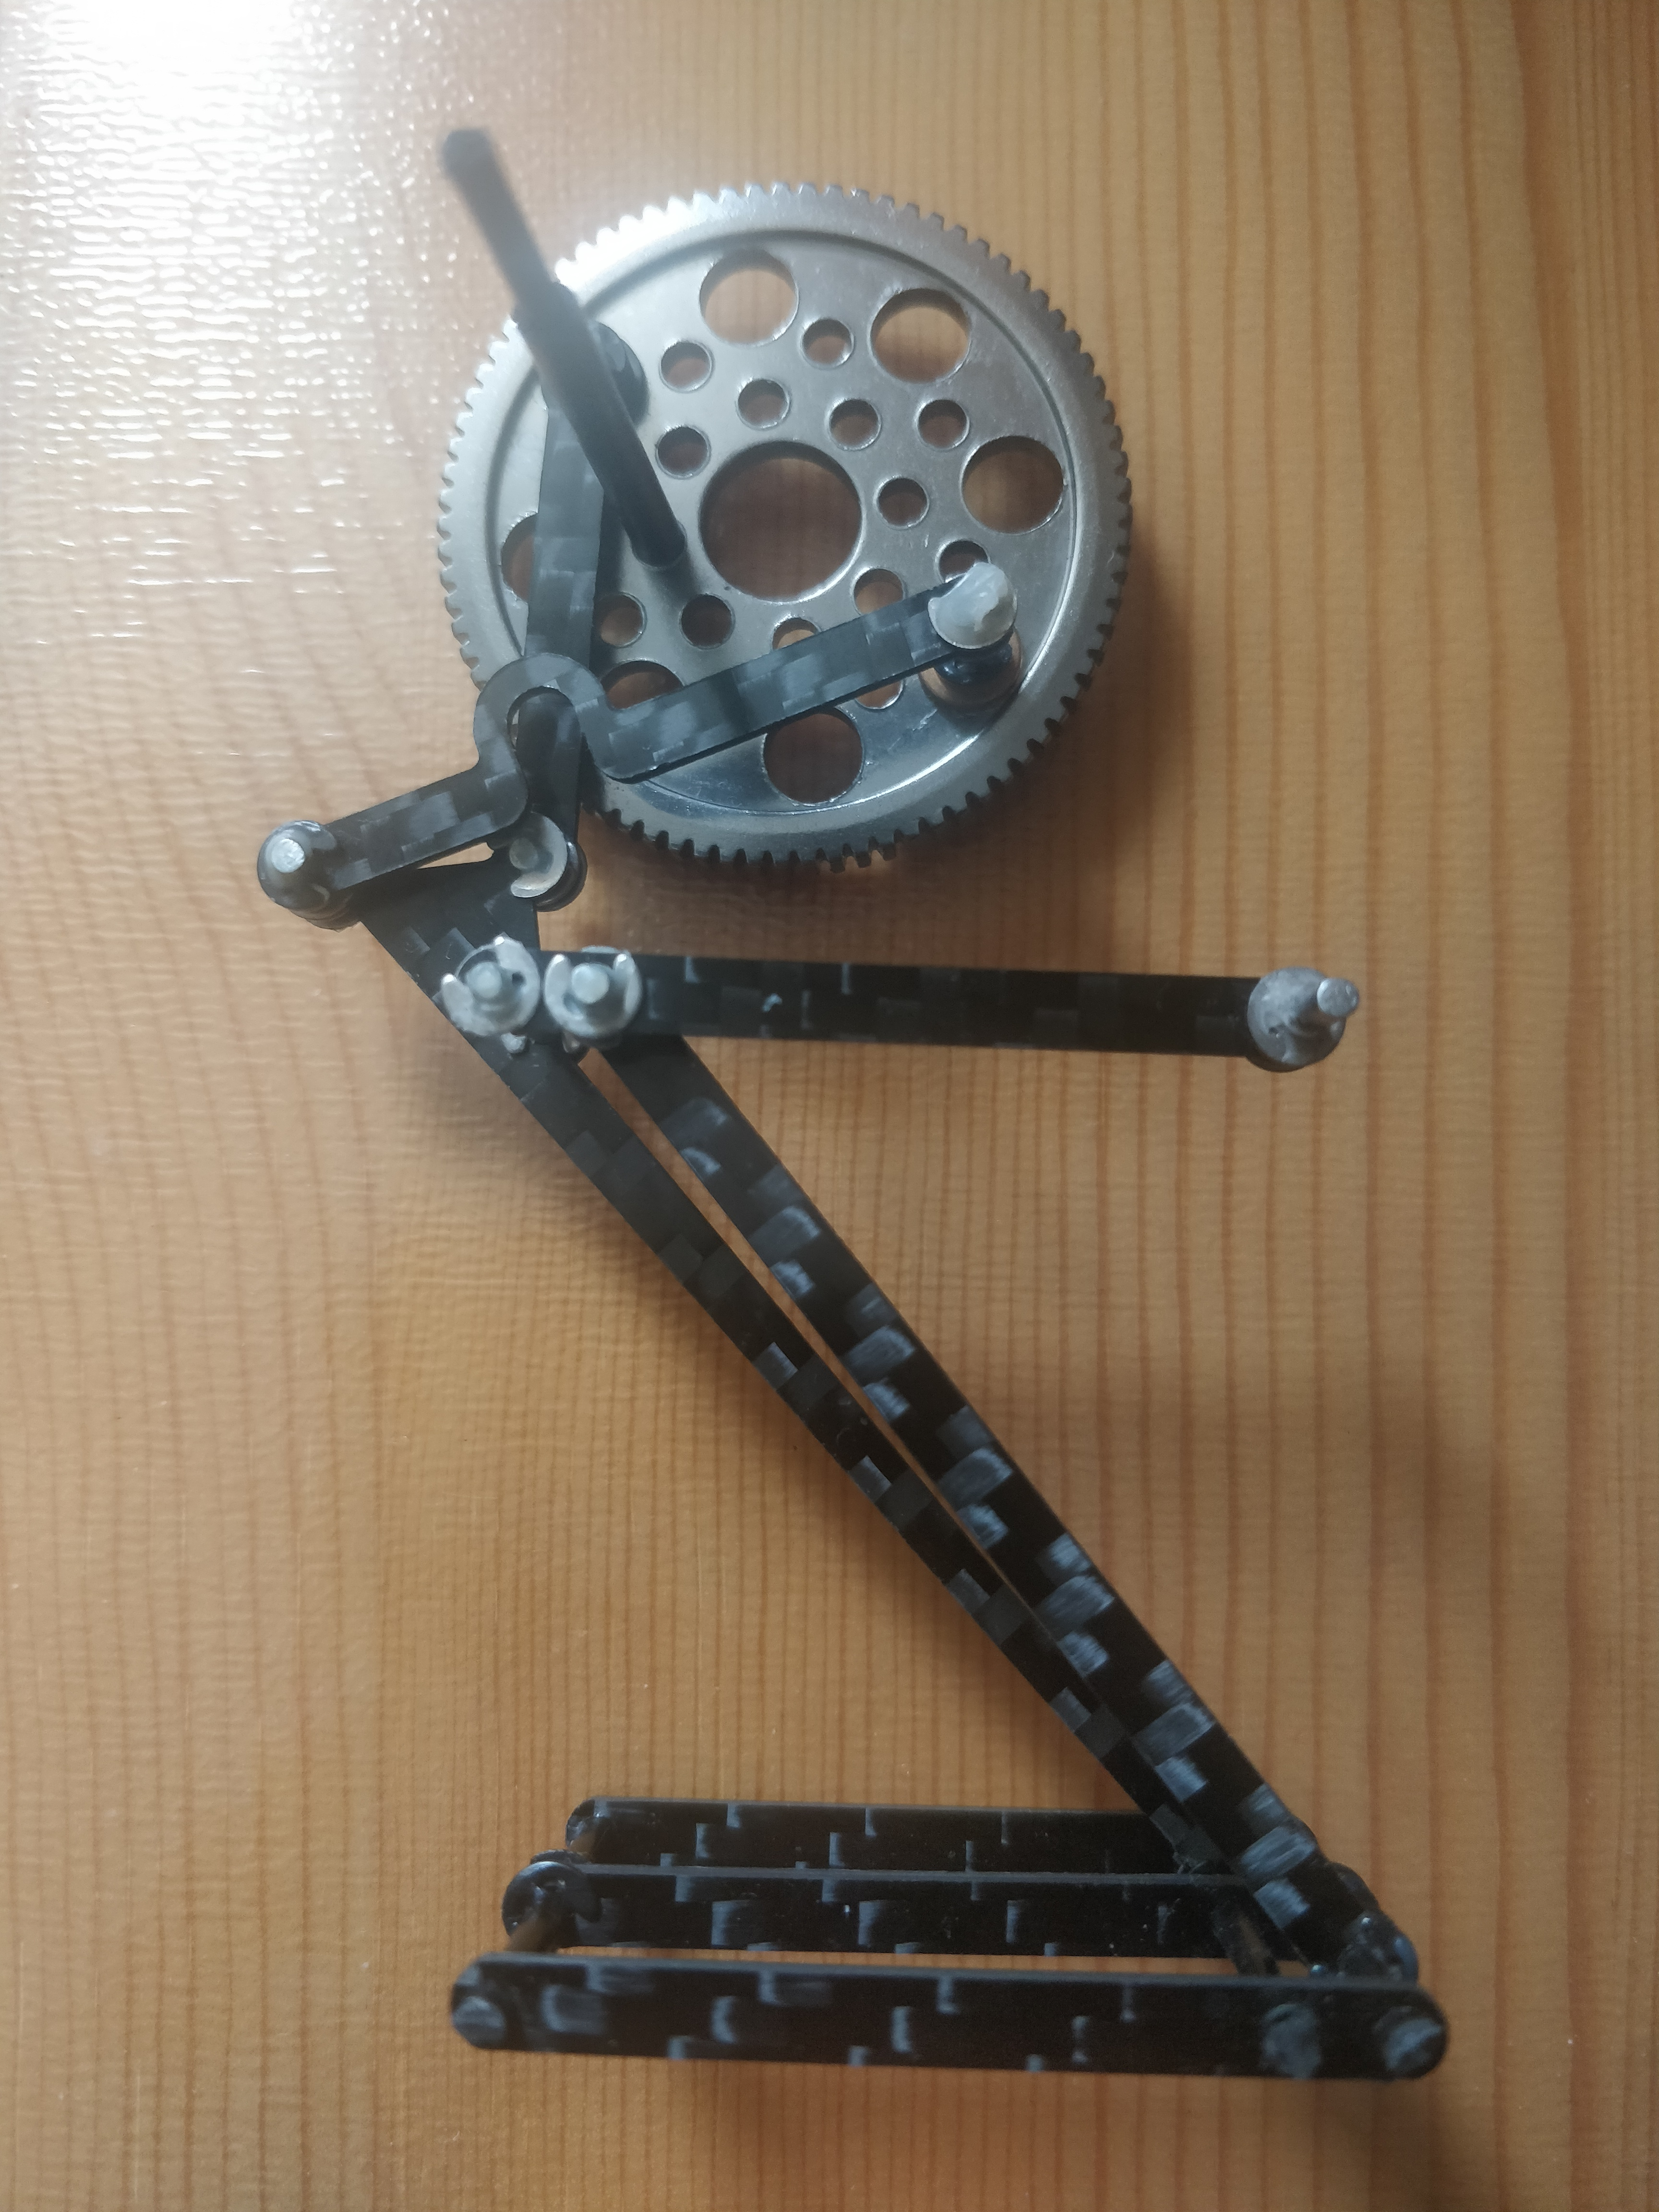
\includegraphics[height=9cm]{leg_assembled.jpeg}
  \caption{AB胶加固后的腿}
  \label{fig:leg_assembled}
\end{figure}
减速器部分同理,次级齿轮用2mm打头轴和卡簧固定,在运动一段时间后卡簧松动,轴会发生歪斜从而导致齿轮卡住。用AB胶固定后改善,如图\ref{fig:retarder_assembled}所示。
\begin{figure}[H]
  \centering%
  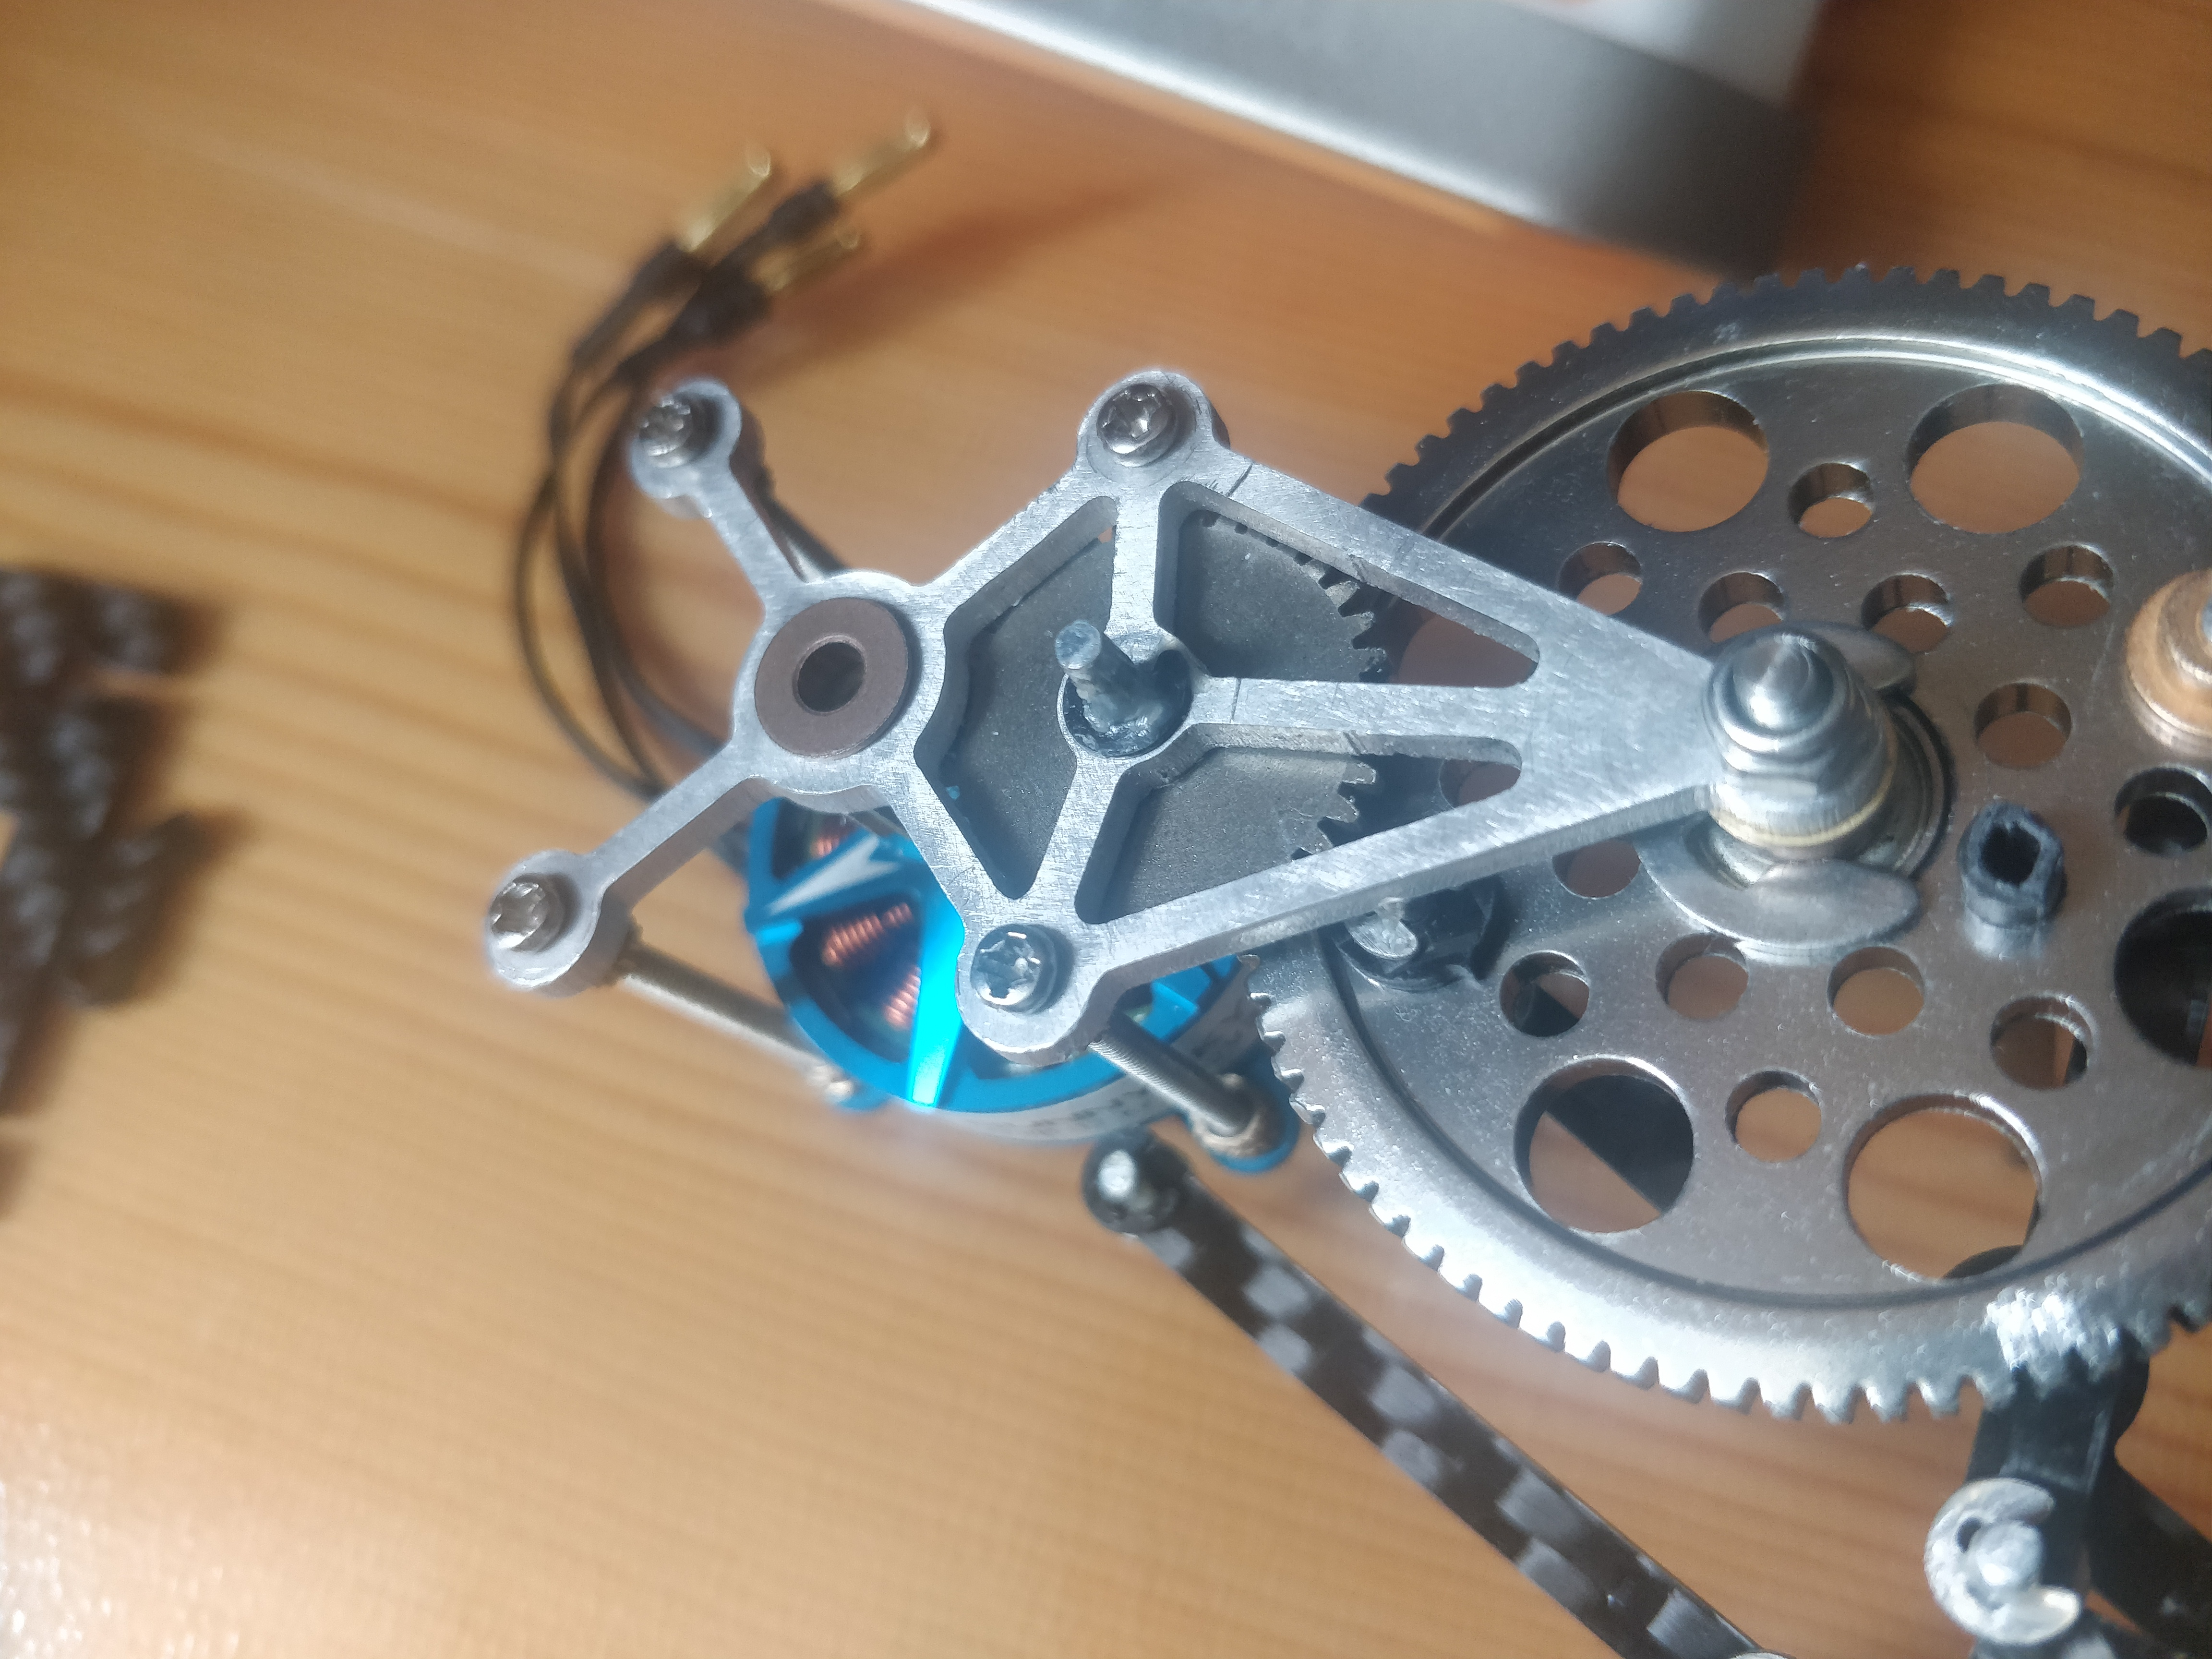
\includegraphics[height=7cm]{retarder_assembled.jpeg}
  \caption{AB胶加固后的减速器}
  \label{fig:retarder_assembled}
\end{figure}
最终组装成品图如图\ref{fig:assembled}所示(未加翼面便于观察):
\begin{figure}[H]
  \centering%
  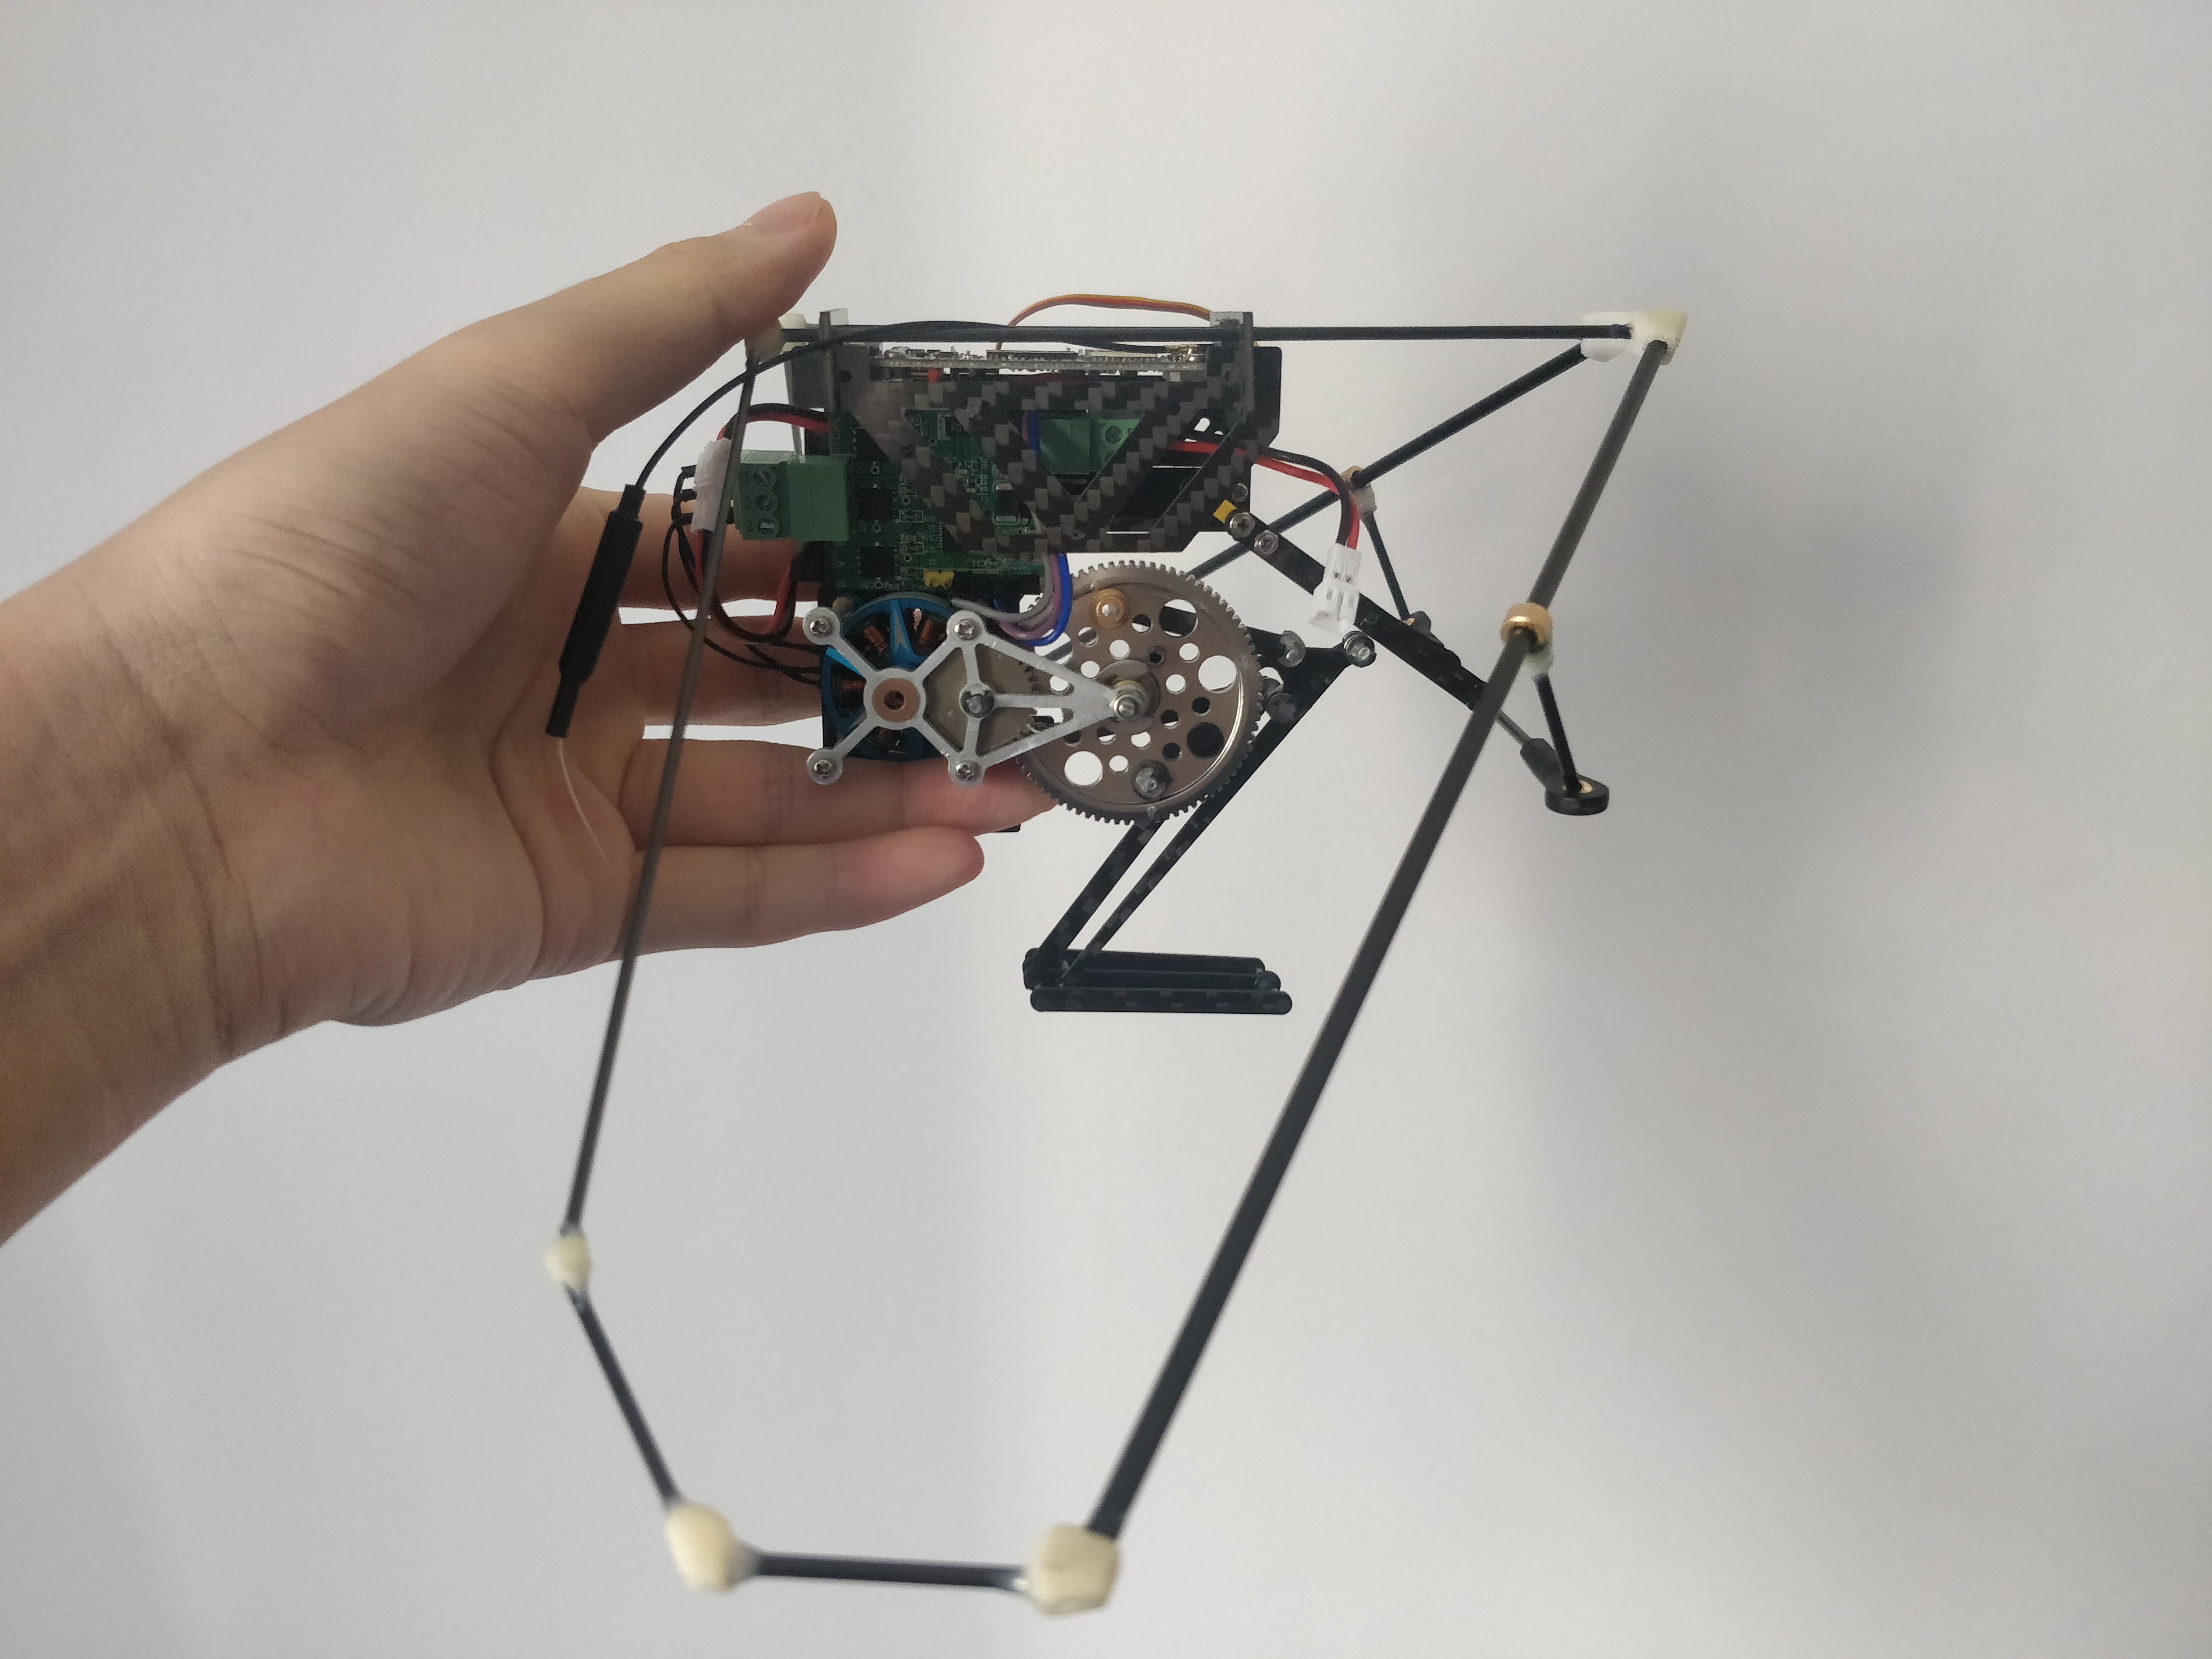
\includegraphics[height=9cm]{assembled.jpeg}
  \caption{组装成品图}
  \label{fig:assembled}
\end{figure}
带翼面的完整版本重量为142g,如图\ref{fig:weight}所示。
\begin{figure}[H]
  \centering%
  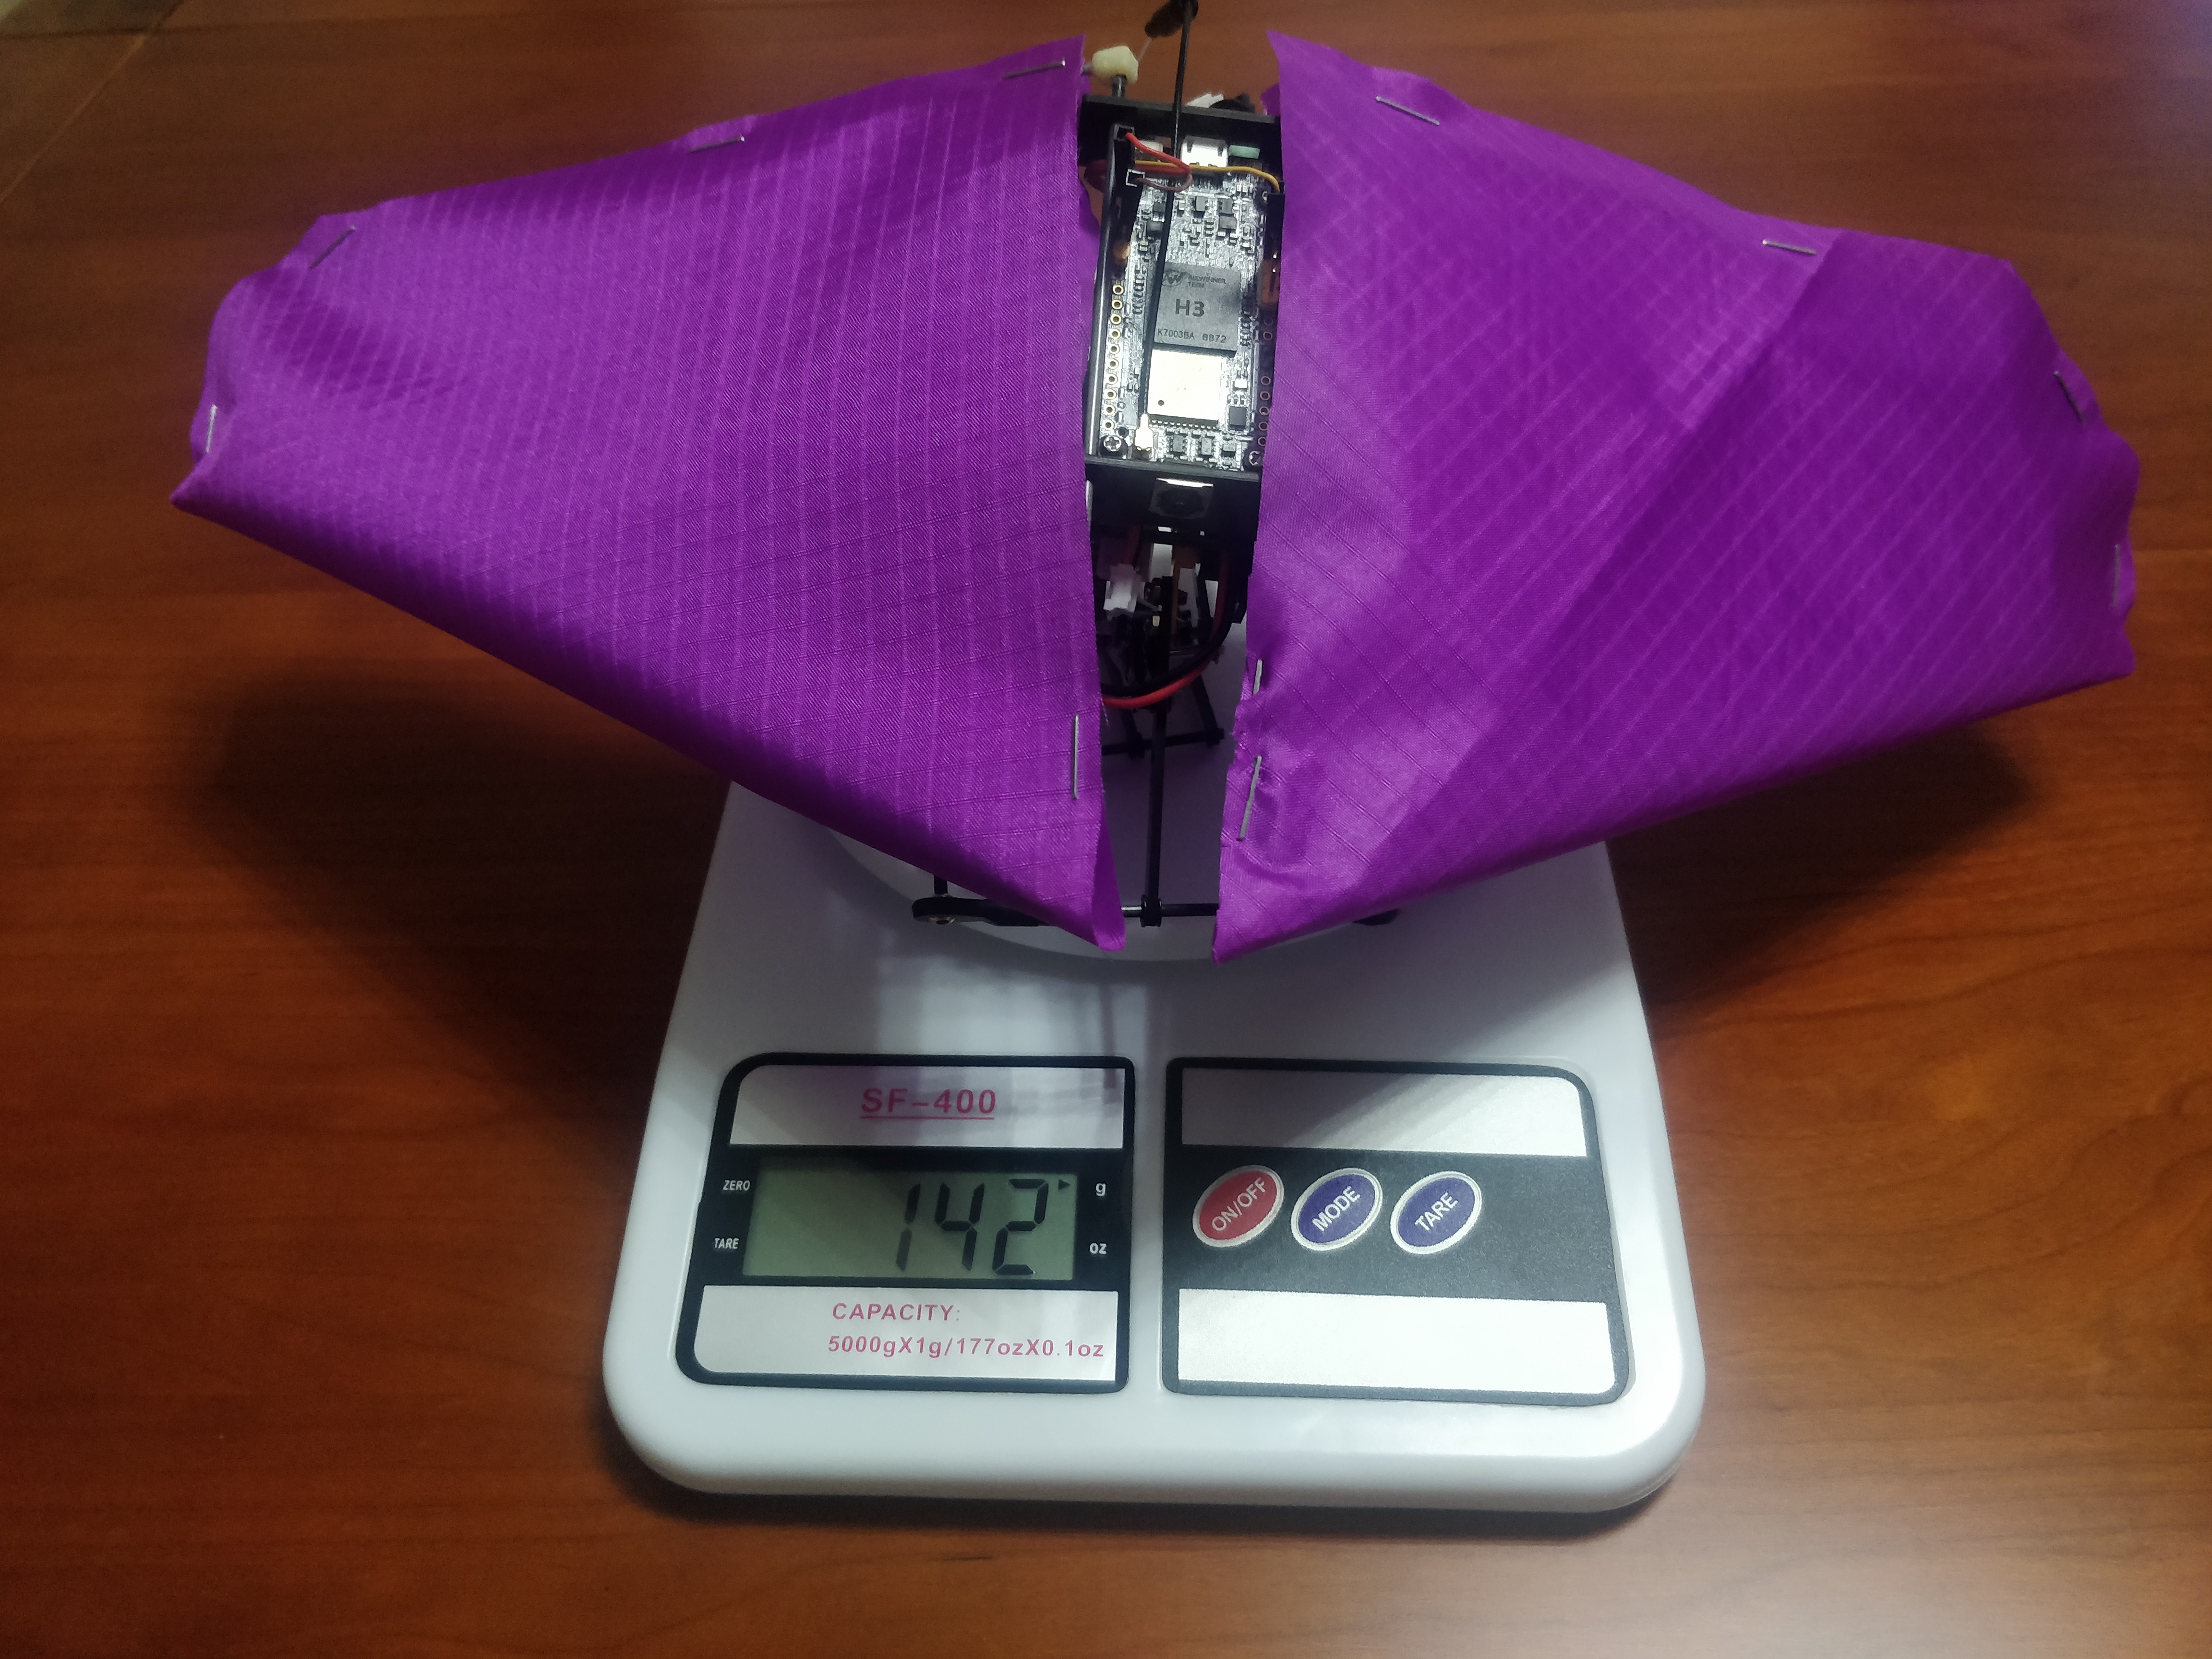
\includegraphics[height=9cm]{weight.jpg}
  \caption{完整版称重}
  \label{fig:weight}
\end{figure}
\section{电机测试}
电机控制测试部分分为空载和带载测试。空载测试配置如图\ref{fig:motor_test}所示。通过改变电机启动电流曲线,进行了平稳启动(2.5s内从0加速至1000rpm)和快速启动(120ms内从0加速至10000rpm)测试,并用MotorControl Workbench自带的画图工具进行了速度监测,得到结果如图\ref{fig:motor_test_speed}所示:

\begin{figure}[H]
  \centering%
  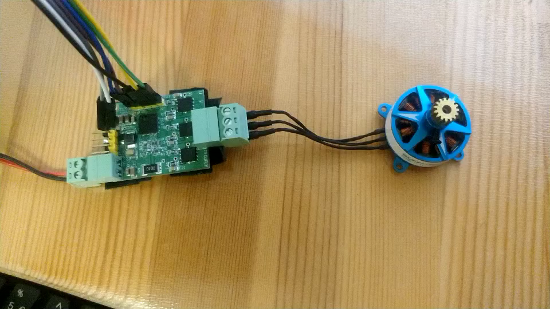
\includegraphics[height=5cm]{motor_test.png}
  \caption{空载配置}
  \label{fig:motor_test}
\end{figure}
\begin{figure}[H]
  \centering
  \subcaptionbox{平稳启动\label{fig:motorspeed1}}[6cm] 
    {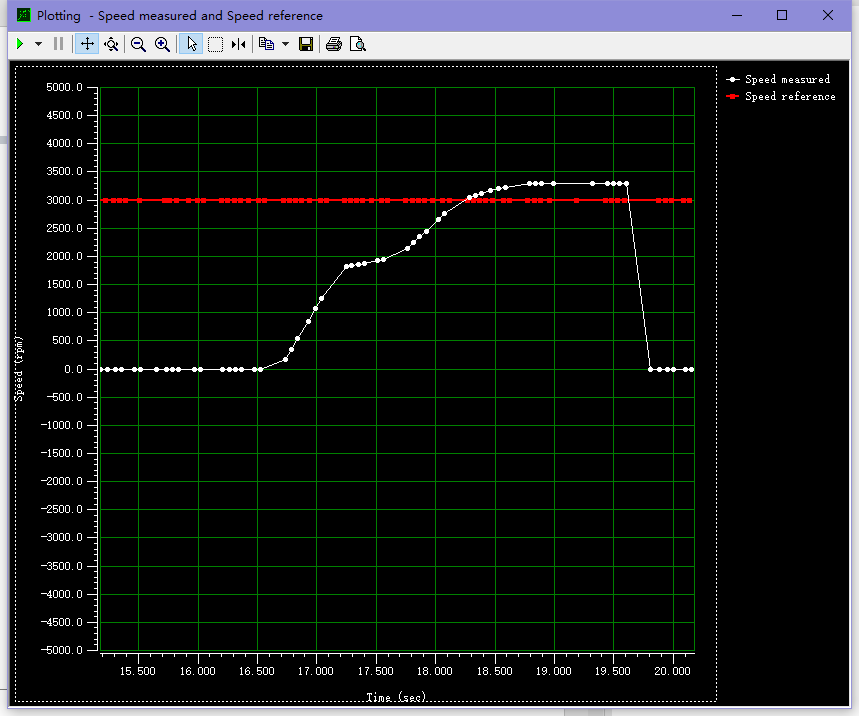
\includegraphics[height=5cm]{motorspeed1.png}}
  \hspace{4em}
  \subcaptionbox{快速启动\label{fig:motorspeed2}}
      {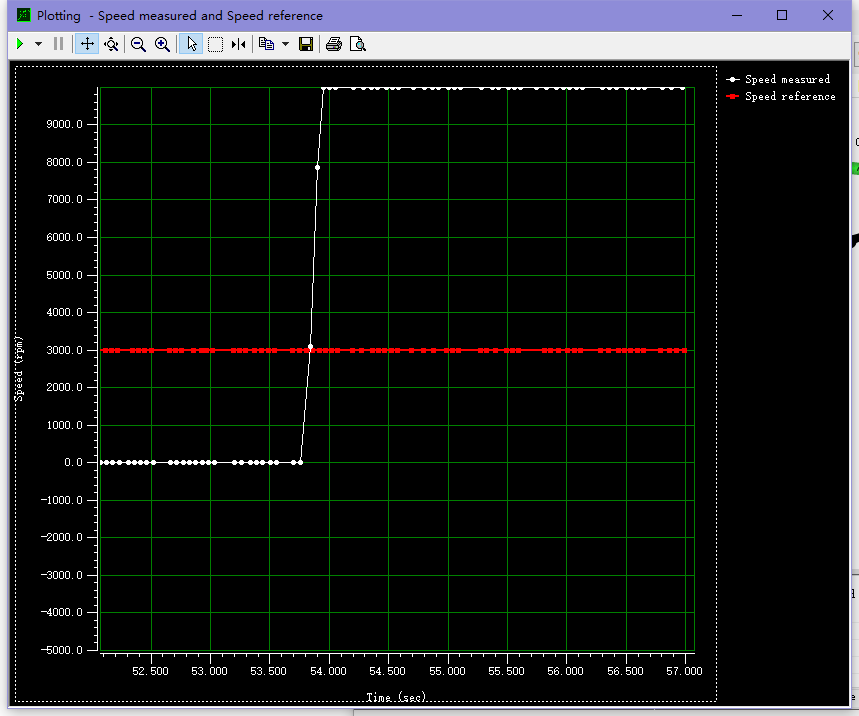
\includegraphics[height=5cm]{motorspeed2.png}}
  \caption{空载测试结果}
  \label{fig:motor_test_speed}
\end{figure}
带载测试配置如图\ref{fig:retarder_test}所示,只安装减速器便于观察输出级齿轮行程,按照同样的参数进行平稳启动和快速启动测试,结果见图\ref{fig:retarder_test_speed}:
\begin{figure}[H]
  \centering%
  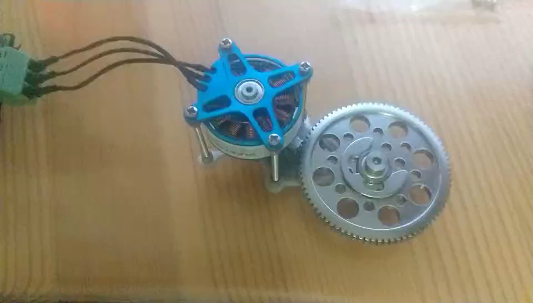
\includegraphics[height=5cm]{retarder_test.png}
  \caption{带载配置}
  \label{fig:retarder_test}
\end{figure}
\begin{figure}[H]
  \centering
  \subcaptionbox{平稳启动\label{fig:motorspeed3}}[6cm] 
    {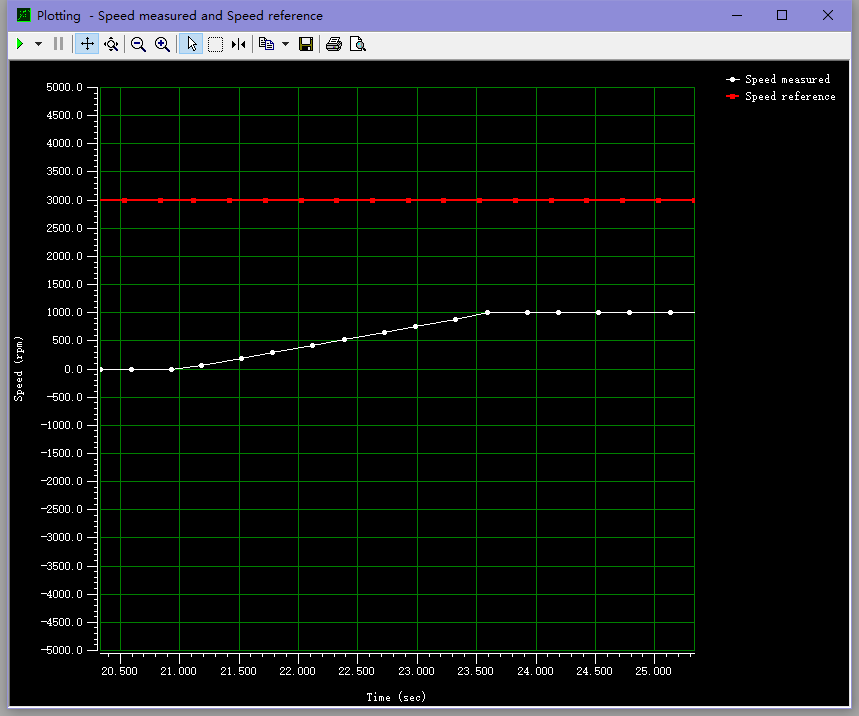
\includegraphics[height=5cm]{motorspeed3.png}}
  \hspace{4em}
  \subcaptionbox{快速启动\label{fig:motorspeed4}}
      {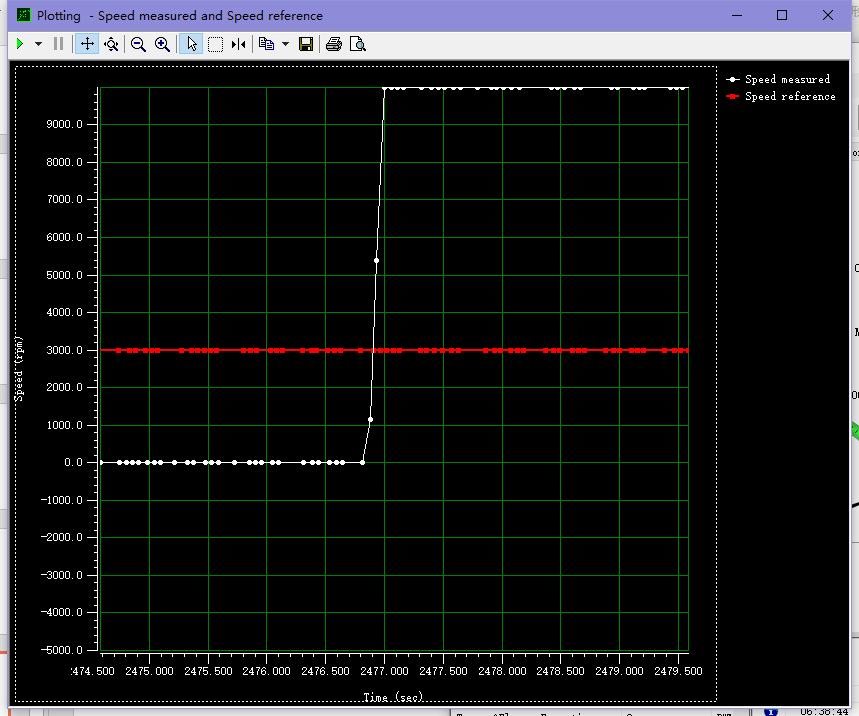
\includegraphics[height=5cm]{motorspeed4.png}}
  \caption{带载测试结果}
  \label{fig:retarder_test_speed}
\end{figure}
测试结果中横坐标为时间(s),纵坐标为转速(rpm),因此启动曲线下方到横轴的面积即为电机行程(转数)。将快速启动曲线近似成直线,则输出级齿轮行程:$$\Theta=\frac{1}{2}\omega_{max}t\div60\div i=0.52(r)$$
大致为半圈,符合设计需求。
\section{机翼测试}
图\ref{fig:wings_test}为机翼测试视频截图:
\begin{figure}[H]
  \centering
  \subcaptionbox{待启动\label{fig:wings_fold}}[6cm] 
    {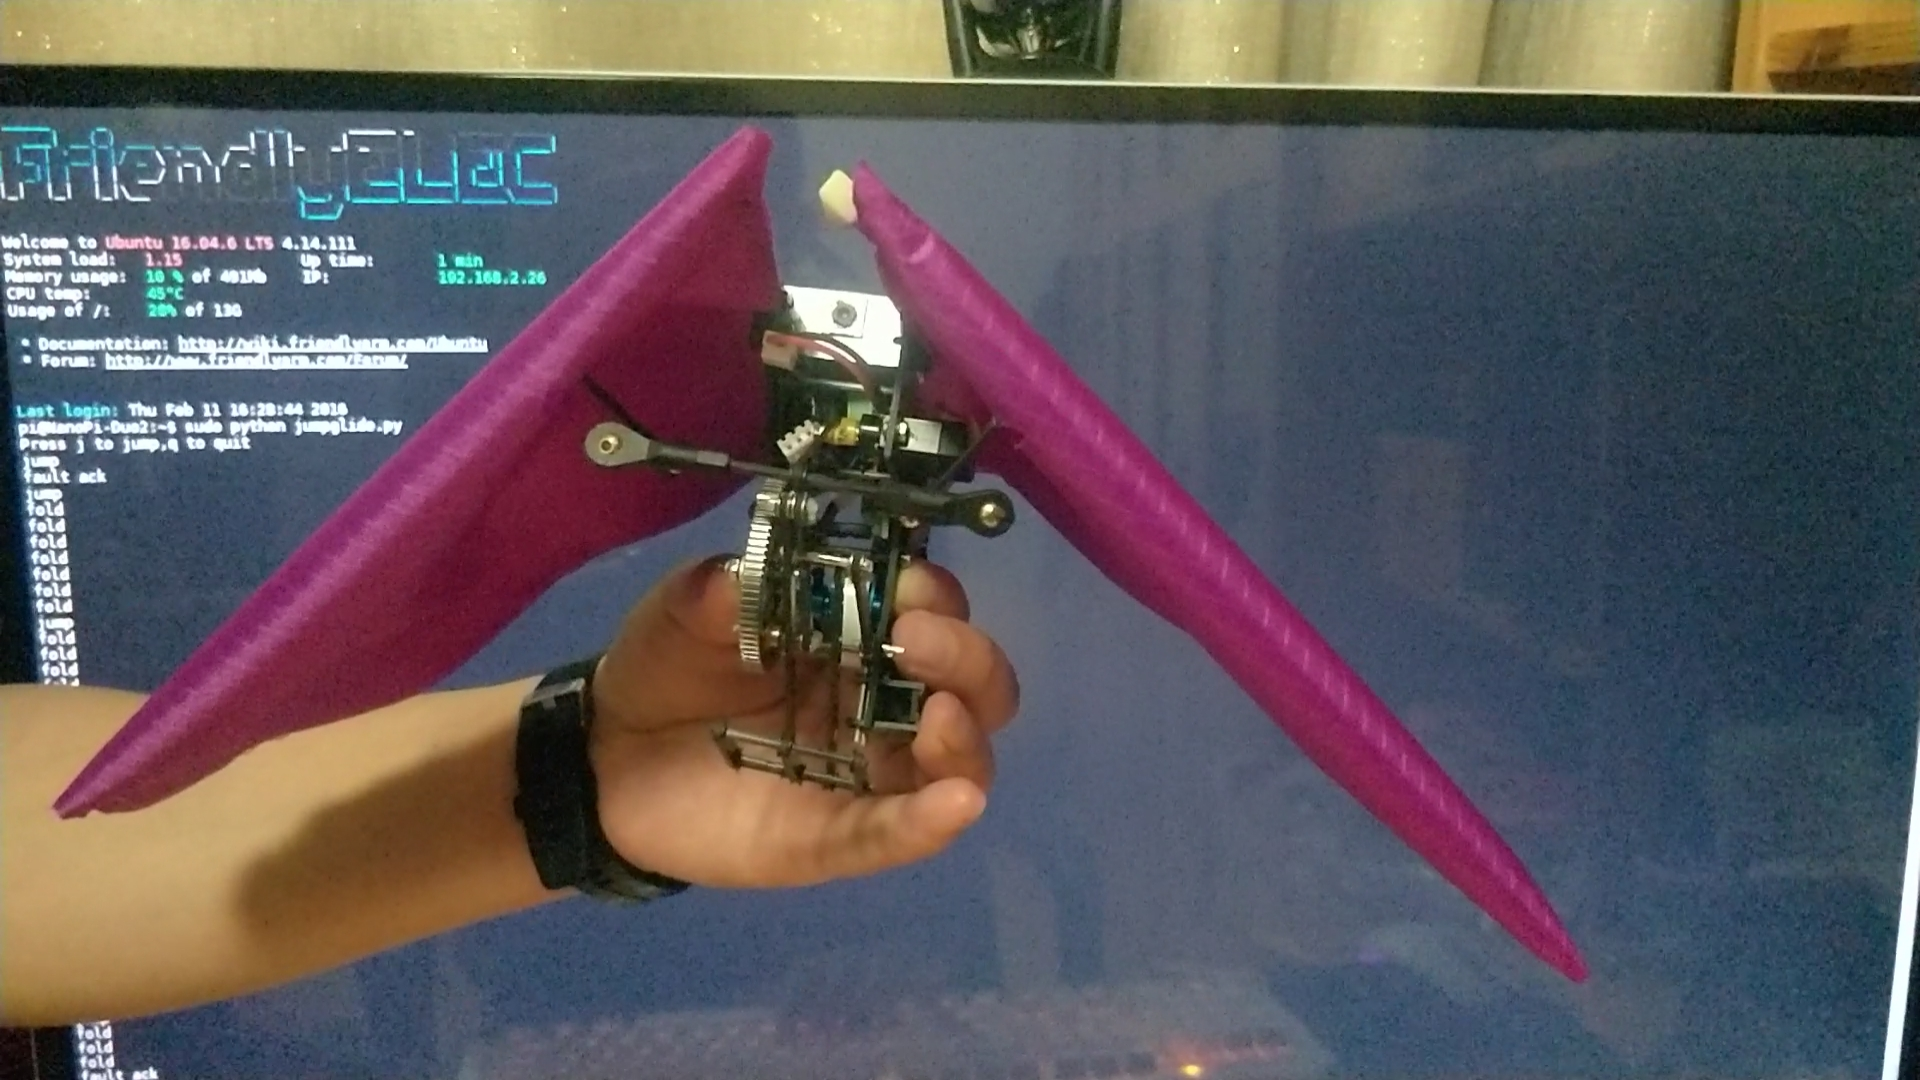
\includegraphics[height=3.5cm]{wings_fold.jpeg}}
  \hspace{4em}
  \subcaptionbox{展平\label{fig:wings_jump}}
      {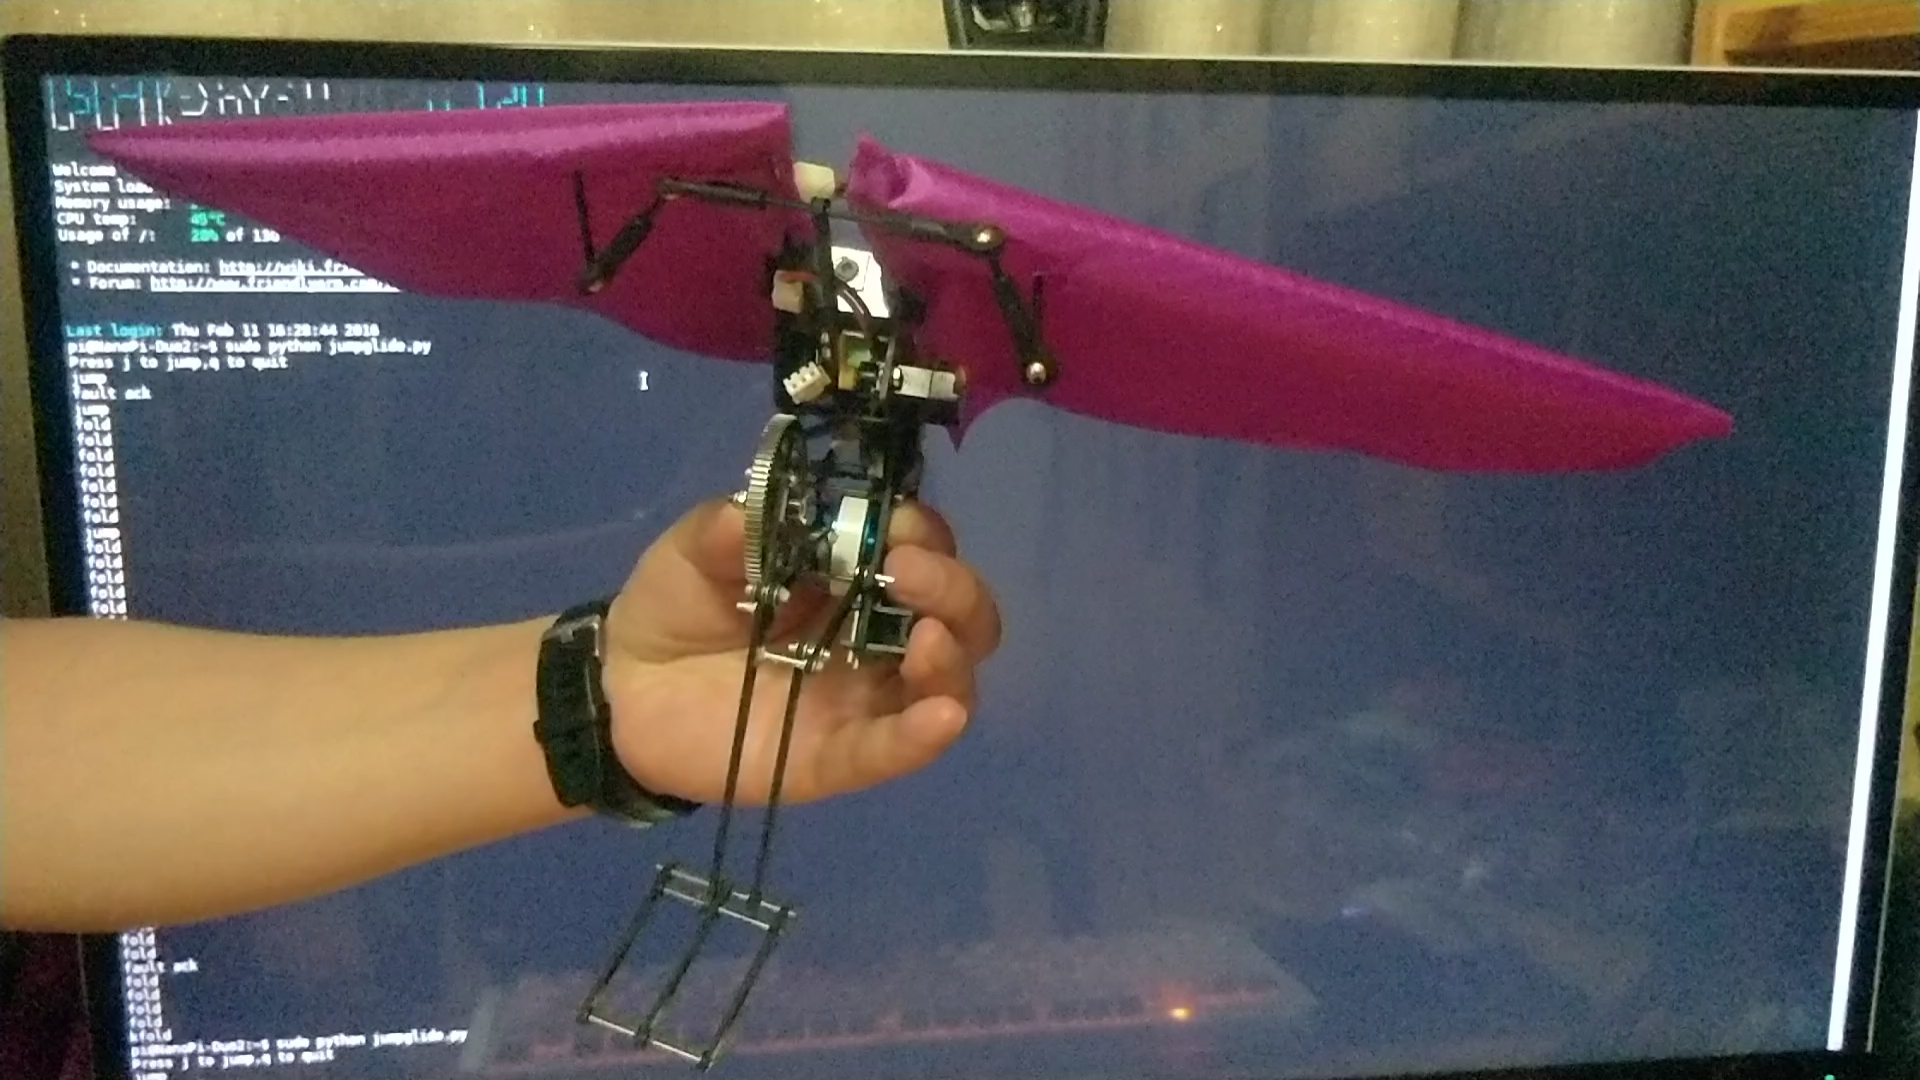
\includegraphics[height=3.5cm]{wings_jump.jpeg}}
  \caption{机翼测试图(截自视频)}
  \label{fig:wings_test}
\end{figure}
通过一个舵机带动,实现了所需的动作。此时的机翼已经与设计图有所区别,由单万向节+滑环变成了双万向节,以避免滑动摩擦力过大的问题。实际结构如图\ref{fig:wings_new}所示。
\begin{figure}[H]
  \centering%
  \includegraphics[height=10cm]{wings_new.jpeg}
  \caption{实际机翼传动结构}
  \label{fig:wings_new}
\end{figure}
\section{跳跃测试}
首先进行空载测试。将机器人侧放在地上,执行跳跃指令,腿部快速打开,证明跳跃机构按设计正常运行。由于动作较快,从录制的视频中截得连续的6帧,如图\ref{fig:jump_test}所示:
\begin{figure}[H]
  \centering
  \subcaptionbox{第0帧\label{fig:jump_test_frame0}}
    {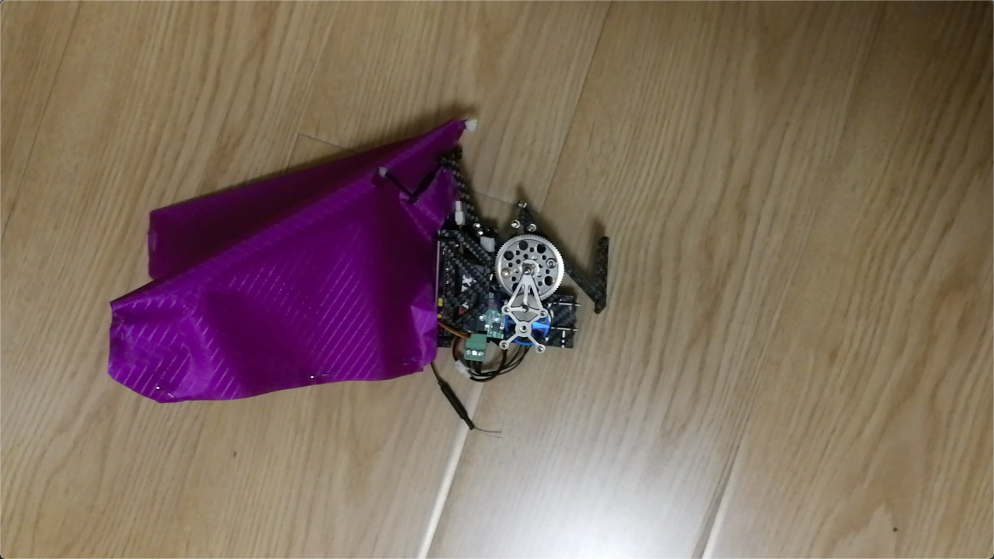
\includegraphics[height=4.5cm,angle=270]{jump_test_frame0.png}}
  % \hspace{4em}
  \subcaptionbox{第1帧\label{fig:jump_test_frame1}}
      {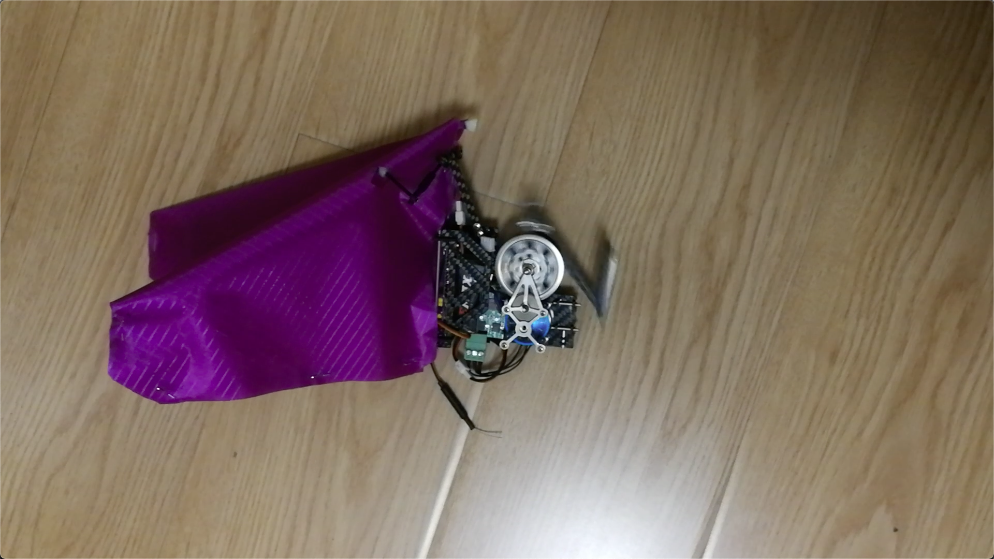
\includegraphics[height=4.5cm,angle=270]{jump_test_frame1.png}}
  % \hspace{4em}
  \subcaptionbox{第2帧\label{fig:jump_test_frame2}}
      {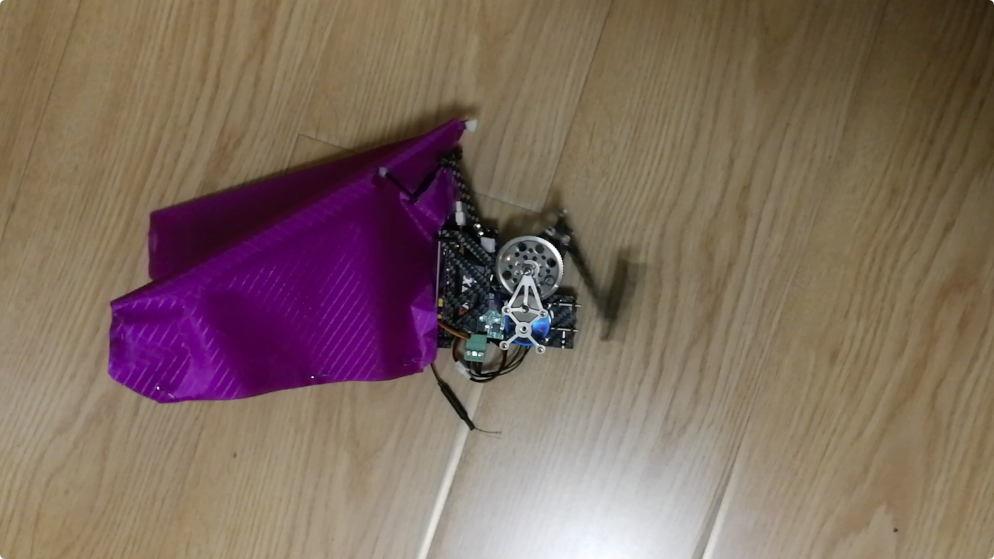
\includegraphics[height=4.5cm,angle=270]{jump_test_frame2.png}}
  % \hspace{4em}
  \subcaptionbox{第3帧\label{fig:jump_test_frame3}} 
      {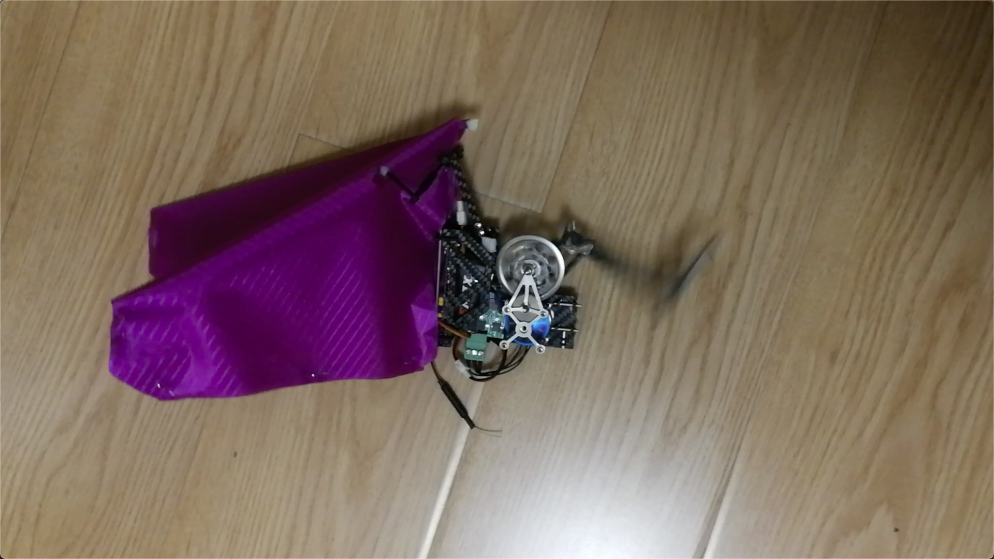
\includegraphics[height=4.5cm,angle=270]{jump_test_frame3.png}}
  % \hspace{4em}
  \subcaptionbox{第4帧\label{fig:jump_test_frame4}} 
      {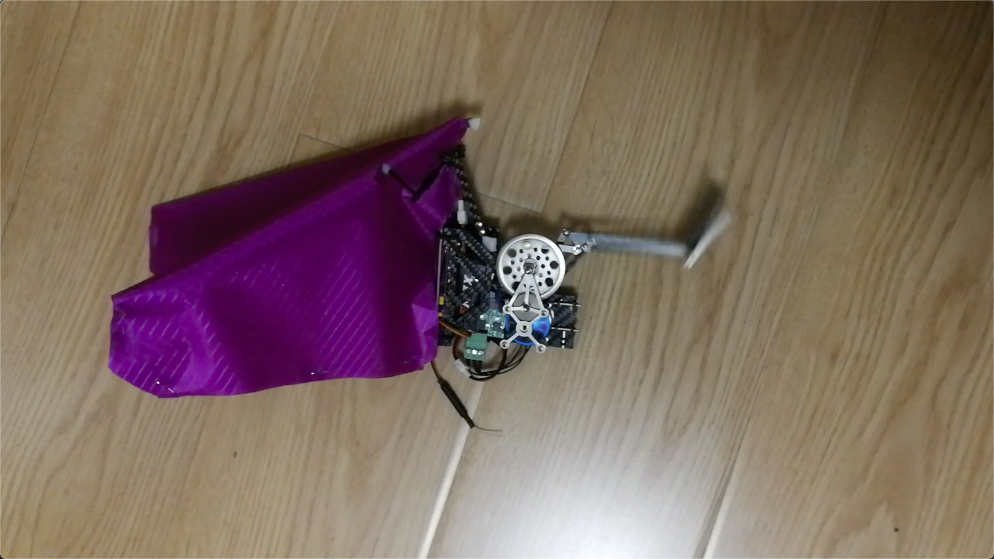
\includegraphics[height=4.5cm,angle=270]{jump_test_frame4.png}}
  % \hspace{4em}
  \subcaptionbox{第5帧\label{fig:jump_test_frame5}}
      {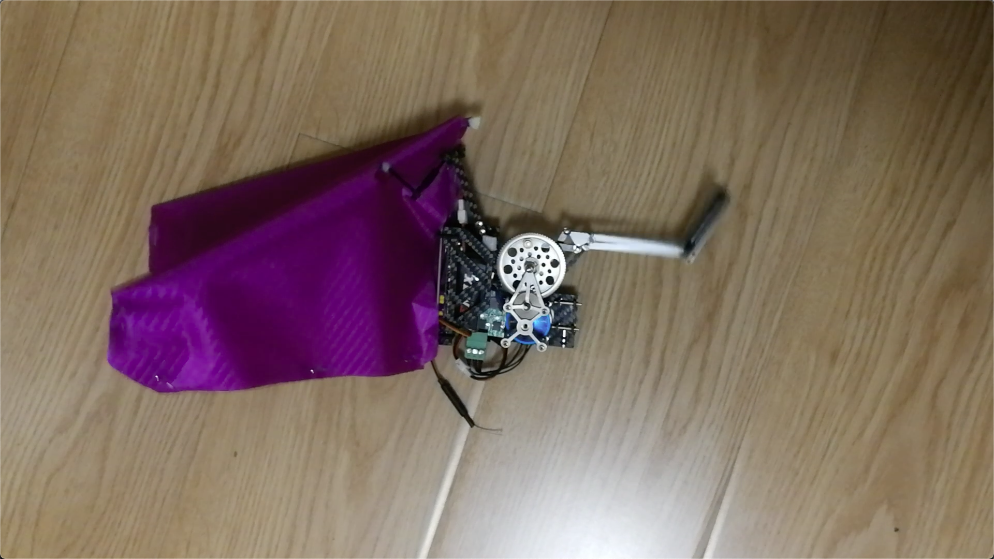
\includegraphics[height=4.5cm,angle=270]{jump_test_frame5.png}}
  \caption{腿测试图(连续6帧)}
  \label{fig:jump_test}
\end{figure}
而在平地起跳测试中,未能成功起跳。如图\ref{fig:failed_test0}所示,机器人蹬出腿后坐在了地上。
\begin{figure}[H]
  \centering
  \subcaptionbox{准备启动\label{fig:failed_start}}[6cm] 
    {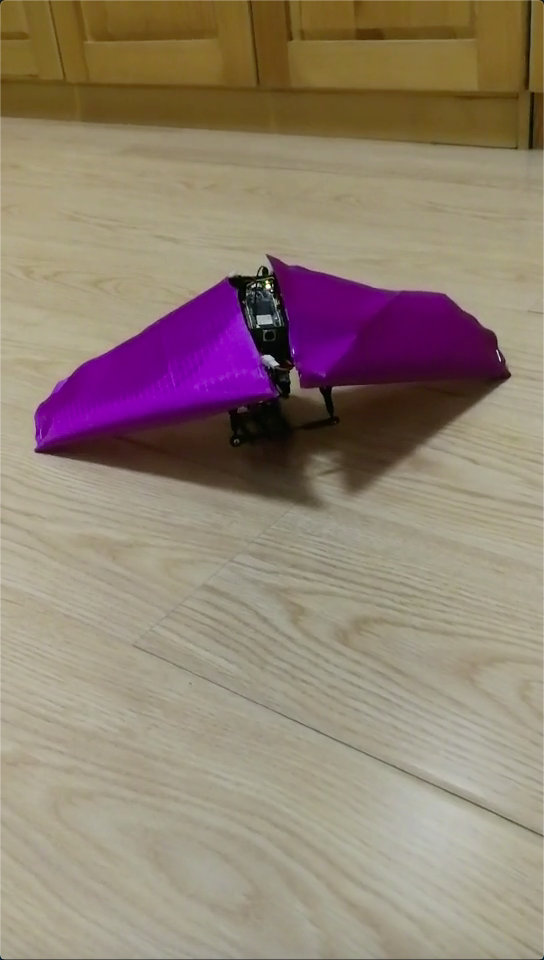
\includegraphics[height=8cm]{failed_start.png}}
  \hspace{4em}
  \subcaptionbox{起跳失败\label{fig:failed_end}}
      {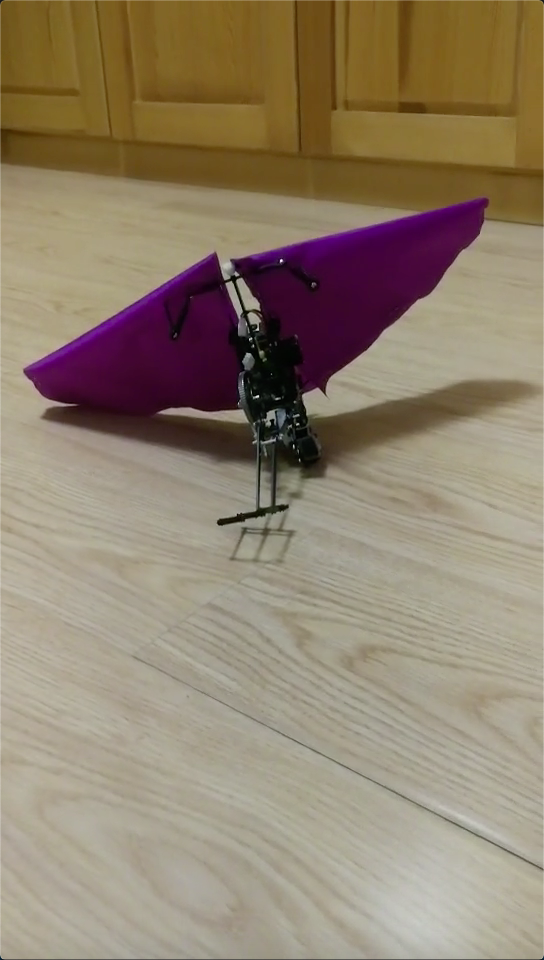
\includegraphics[height=8cm]{failed_end.png}}
  \caption{平地起跳测试}
  \label{fig:failed_test0}
\end{figure}
考虑到重心位置问题,将机器人放在前倾的斜坡上再进行测试,如图\ref{fig:failed_test1}所示。
\begin{figure}[H]
  \centering
  \subcaptionbox{准备启动\label{fig:failed_start2}}[6cm] 
    {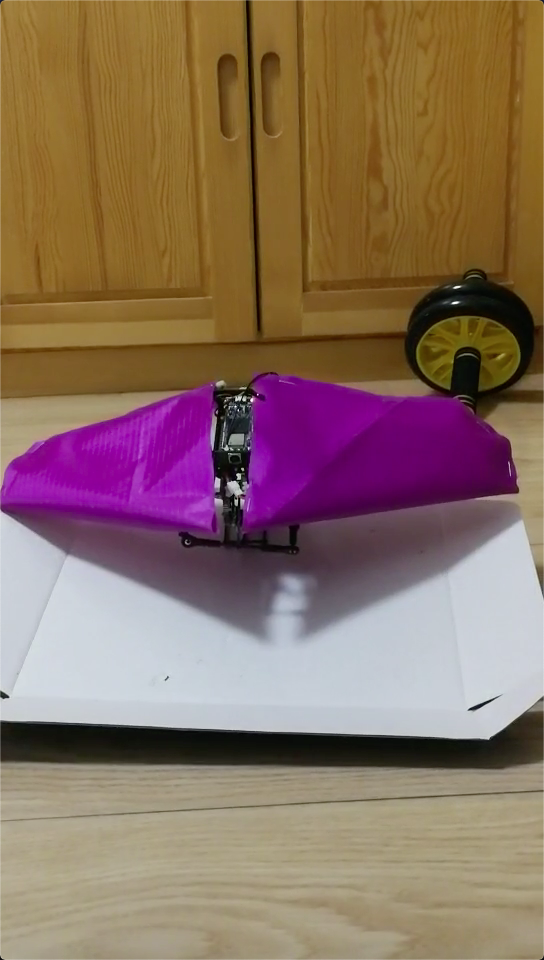
\includegraphics[height=8cm]{failed_start2.png}}
  \hspace{4em}
  \subcaptionbox{起跳失败\label{fig:failed_end2}}
      {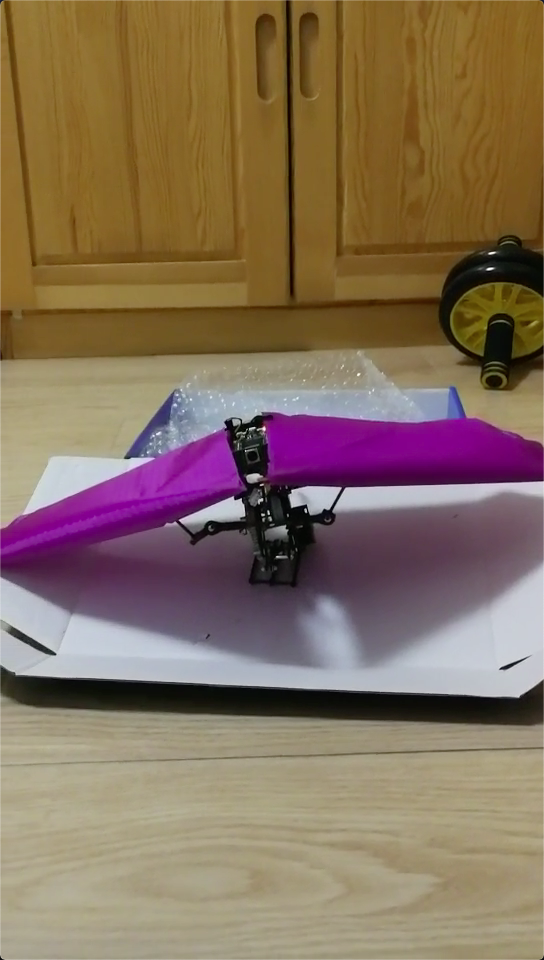
\includegraphics[height=8cm]{failed_end2.png}}
  \caption{斜坡起跳测试}
  \label{fig:failed_test1}
\end{figure}
这次机器人能够保持身体平衡,但腿并未完全展开就停止了。说明电机并未完成所需位移。推测由于所受力矩的变化,开环控制的电机启动过程不能保证对转子位置估计的准确性,因此电机加速失败。而闭环启动需要外接霍尔传感器,需要对机械结构做出较大改变,由于时间所限,遗憾未能实现。且腿部的连接部分的晃动也使得电机的力矩不能有效地传递到与地面接触点,因此理想方案应当对整个腿部进行重新设计,更换材料并设计更可靠的连接方式。以及身体重心的控制,都是本项目的可改进方向。

